\appendix

\section{Additional Background and Preliminaries}\label{sec:literature-appendix}

\paragraph{Backward unmasking process of MDMs.}
It is known that the time reversal of a CTMC with rate $Q_t$ is also a CTMC, whose infinitesimal transition probability takes a form analogous to \eqref{eq:infinitesimal_transition}:
\begin{equation}
\label{eq:infinitesimal_transition_rev}
    q_{t-\Delta t|t}(\vy|\vx_t)  =  \delta(\vx_t, \vy) + \tilde{Q}_t(\vx_t, \vy) \Delta t + o(\Delta t).
\end{equation}
Here, $\tilde Q_t$ is an unknown transition rate. Specifically for MDMs, the reverse transition is an unmasking process \citep{lou2024discrete,campbell2022continuous,ou2025absorbingdiscretediffusionsecretly}, where we begin from an all-mask sequence and randomly unmask each to a token in the vocabulary with the following token level transitions:
\begin{align*}
    q_{s|t}\!\left(x_s^{i}|\bm x_t\right)
=
&\quad \begin{cases}
1,
& x_t^{i} \neq \mask,\; x_s^{i} = x_t^{i}, \\
\dfrac{1 - e^{-\bar{\sigma}(s)}}{1 - e^{-\bar{\sigma}(t)}},
& x_t^{i} = \mask,\; x_s^{i} = \mask, \\
\dfrac{e^{-\bar{\sigma}(s)} - e^{-\bar{\sigma}(t)}}{1 - e^{-\bar{\sigma}(t)}}\,
q_{0 | t}\!\left(x_s^{i}|x_t\right),
& x_t^{i} = \mask,\; x_s^{i} \neq \mask, \\
0,
& \text{otherwise}.
\end{cases}
\end{align*}
Therefore, the learning of the backward process reduces to the learning of the reverse rate $\tilde Q_t$ parameterized by a neural network with weight $\theta$. The training can be implemented by various approaches, such as by minimizing score-based objectives \citep{lou2024discrete,ou2025absorbingdiscretediffusionsecretly}. In this way, we have a parameterized approximation of the true backward rate $P_t^\theta\approx \tilde Q_t$, which leads to a marginal distribution $p_t^\theta$ at time $t$ by solving the Kolmogorov ODE $dp^\theta_t/dt=p_t^\theta P_t^\theta$.

\paragraph{Trainable inference methods for MDMs.}
Beyond fixed heuristics, several works treat the unmasking order as a trainable policy. Some introduce a separate policy network to learn update sequences \citep{peng2025path, jazbec2025learning, chen2025dultra} or introduce an additional MDM training stage on the preferred trajectories \citep{song2025seeddiffusionlargescalediffusion}, while others modify the backward process itself to encourage more structured updates, such as jointly updating semantically related variables \citep{meshchaninov2025guided} or incorporating corrective refinement steps for already unmasked tokens \citep{zhao2024informed}. These methods demonstrate that learning the inference procedure can significantly improve sample quality, but most existing approaches rely on rewards (reinforcement learning) or ad hoc update rules. Based on sample likelihood maximization, \citet{wang2025learningorder} proposes a framework to learn the optimal decoding order for any-order autoregressive models \citep{shih2022traininginferenceanyorderautoregressive}, which are limited to single-token generation processes; our \alg{} extends this framework to multi-token unmasking in masked diffusion models. From a related likelihood-based perspective, \citet{turok2026duel} restrict attention to deterministic position selection and obtain exact test-time likelihoods within this class. 

\section{Proofs}
\subsection{Preparation}
Consider an indexing of subsets $j\mapsto\mathcal U_j$ for all the size-$N$ subsets $\mathcal U_j$ of $[L]$. We denote $\bm\pi\in\mathbb R^{\binom{L}{N}}$ a probability vector such that $\pi_j:=\pi(\mathcal U_j|\bm x_k)$. Similarly, we denote $\bm z\in\mathbb R^{\binom{L}{N}}$ a random vector such that $z_j:=\prod_{i\in\mathcal U_j}p_{t_k}^{\theta,\pi}(x^i|\bm x_k)$, with the randomness $x^i\sim p_{t_k}^{\theta,\pi}(\cdot|\bm x_k)$. Then, \eqref{eq:trainable_confidence} becomes the following optimization problem over the probability simplex $\Delta$:
\begin{align}\label{eq:obj-equiv}
    \min_{\bm\pi\in\Delta}f(\bm\pi):=-\EE\log(\bm z^\top\bm\pi).
\end{align}

\subsection{Proof of Theorem \ref{thm:confidence}}\label{subsec:proof-confidence}
\begin{proof}
\textbf{Condition (1).} If $\pi$ is restricted to be a deterministic policy, then the optimal $\bm\pi^*=\bm e_j$ for some standard basis vector $\bm e_j$. Taking this to \eqref{eq:obj-equiv}, 
\begin{align*}
f(\bm\pi^*)&=-\EE\log z_j=-\EE_{\bm x\sim p_{t_k}^\theta(\cdot|\bm x_k)}\log\prod_{i\in\mathcal U_j}p_{t_k}^\theta(x^i|\bm x_k)\\
&=-\sum_{i\in\mathcal U_j}\sum_{v\in\mathcal V} p_{t_k}^\theta(x^i=v|\bm x_k)\log p_{t_k}^\theta(x^i=v|\bm x_k)=\sum_{i\in\mathcal U_j}H_k(i).
\end{align*}
Therefore, the minimum must be attained at the policy that deterministically outputs $\mathcal U^*$ with the smallest total entropy.

\textbf{Condition (2).} By \citet{cover1987log}, the KKT optimality conditions state that for an optimal $\bm\pi^*$,
\begin{align*}
    \EE\left[\frac{z_j}{\bm z^\top\bm\pi^*}\right]\begin{cases}
        =1,&\text{if }\bm\pi^*_j>0,\\
        \leq1,&\text{if }\bm\pi^*_j=0.
    \end{cases}
\end{align*}
Thus, if $\bm e_k$ is optimal for some $k$, then $\EE[z_j/z_k]\leq1$ for all $j$. Moreover, since there exists strictly feasible $\bm\pi$ in the probability simplex, Slater's condition holds and KKT optimality is necessary and sufficient. Thus an optimal $\bm\pi^*$ must be deterministic, and we have the same result as in Condition (1).

\end{proof}

\begin{remark}
A related entropy criterion appears independently in \citet{benhamu2025eb}: their EB-Sampler unmasks token subsets satisfying an entropy-difference bound $\sum_{l\in\mathcal U}H_k(l)-\max_{l\in\mathcal U}H_k(l)\leq\gamma$, motivated as an upper bound on joint dependence error in a KL-based analysis of MDM sampling. Theorem~\ref{thm:confidence} provides a complementary justification: under our locality restriction, entropy-greedy unmasking is the optimal stochastic policy for likelihood maximization, giving a likelihood-theoretic foundation for the use of entropy as the unmasking signal.
\end{remark}

\begin{remark}
The optimization framework underlying Theorem~\ref{thm:confidence} naturally extends to other confidence-based heuristic samplers by augmenting \eqref{eq:trainable_confidence} with additional data-dependent constraints on the policy. Provided such constraints act separably on the feasible simplex of $\pi(\cdot|\bm x_k)$ and preserve convexity, the KKT analysis carries through on the restricted region, and the optimal policy reduces to entropy-greedy unmasking within the constrained subset. We illustrate this with KLASS \citep{kim2025klass} in Appendix~\ref{subsec:klass-extension}.
\end{remark}

\subsection{Worked Example: KLASS as a Constrained Instance}\label{subsec:klass-extension}

We illustrate how the framework underlying Theorem~\ref{thm:confidence} extends to other confidence-based heuristic samplers, using KLASS \citep{kim2025klass} as a representative example. KLASS augments confidence unmasking with a KL-stability filter: at each step $k$, it scores each masked position by the KL divergence between the predicted vocabulary distribution at $\bm x_k$ and predictions from a recent history window, and restricts unmasking to the stable subset
\begin{align*}
    S_k = \{i \in [L] : x_k^i = \mask,\ \text{position } i \text{ is KL-stable over the history window}\} \subseteq [L].
\end{align*}
Within this stable set, KLASS unmasks the highest-confidence positions.

In our framework, this restriction amounts to constraining the support of $\pi(\cdot | \bm x_k)$ to subsets $\mathcal U \subseteq S_k$. Following the indexing of Appendix~\ref{subsec:proof-confidence}, let $J(S_k) := \{j : \mathcal U_j \subseteq S_k\}$, and let
\begin{align*}
    \Delta_{S_k} := \{\bm\pi \in \Delta : \pi_j = 0 \text{ for all } j \notin J(S_k)\}
\end{align*}
denote the induced sub-simplex. The KLASS-constrained version of \eqref{eq:trainable_confidence} is then
\begin{align}\label{eq:klass-obj}
    \min_{\bm\pi \in \Delta_{S_k}} f(\bm\pi) = -\EE\log(\bm z^\top \bm\pi),
\end{align}
which differs from \eqref{eq:obj-equiv} only in its feasible set.

\begin{proposition}\label{prop:klass}
Under the conditions of Theorem~\ref{thm:confidence}, with $|S_k| \geq N$, the optimal solution to \eqref{eq:klass-obj} is $\bm\pi^* = \bm e_{j^*}$ where
\begin{align*}
    \mathcal U^* = \argmax_{\mathcal U \subseteq S_k,\, |\mathcal U| = N} \sum_{i \in \mathcal U} -H_k(i),
\end{align*}
recovering the unmasking rule of KLASS.
\end{proposition}

\begin{proof}
$\Delta_{S_k}$ is itself a probability simplex, supported on $J(S_k)$. The KKT analysis in the proof of Theorem~\ref{thm:confidence} applies verbatim with the index $j$ ranging over $J(S_k)$ rather than the full set, since the stationarity condition is separable across coordinates and the constraint $\bm\pi \in \Delta_{S_k}$ preserves convexity. The optimum is therefore attained at a vertex $\bm e_{j^*}$, with $j^*$ corresponding to the size-$N$ subset $\mathcal U^* \subseteq S_k$ that minimizes the total entropy $\sum_{i \in \mathcal U} H_k(i)$.
\end{proof}

The same reduction applies to any confidence-based sampler that imposes a data-dependent feasibility set $\mathcal U \in \mathcal C(\bm x_k)$ determined by the model's predictions (and not by $\pi$ itself). In each case, the optimal policy under the constrained objective is the entropy-greedy choice within $\mathcal C(\bm x_k)$.

\subsection{Proof of Theorem~\ref{thm:confidence-rand}}\label{subsec:proof-random}
\begin{proof}
The Hessian of the objective is
\begin{align*}
    \nabla^2f(\bm\pi)=\EE\left[\frac{\bm z\bm z^\top}{(\bm z^\top\bm\pi)^2}\right]\succeq\EE[\bm z\bm z^\top]=\bm\Sigma,
\end{align*}
for $(\bm z^\top\bm\pi)^2\leq\|\bm z\|_\infty^2\leq1$. Therefore, $\nabla^2f(\bm\pi)$ is positive-definite with smallest eigenvalue greater than $\lambda=\lambda_{\min}(\bm\Sigma)$. This means $f$ is $\lambda$-strongly convex, i.e. for any $\bm\pi,\bm\pi'$,
\begin{align*}
    f(\bm\pi)-f(\bm\pi')\geq\ip{\nabla f(\bm\pi'),\bm\pi-\bm\pi'}+\frac{\lambda}{2}\nm{\bm\pi-\bm\pi'}^2_2.
\end{align*}
Denoting $\hat{\bm\pi}=\bm e_{j^*}$ for $j^*$ corresponding to $\mathcal U^*$. By the above inequality we have
\begin{align}
    f(\hat{\bm\pi})-f(\bm \pi^*)&\leq\ip{\nabla f(\hat{\bm\pi}),\hat{\bm\pi}-\bm\pi^*}-\frac{\lambda}{2}\nm{\hat{\bm\pi}-\bm\pi^*}^2_2\nonumber\\
    &=\ip{\bm P\nabla f(\hat{\bm\pi}),\hat{\bm\pi}-\bm\pi^*}+\ip{\nabla f(\hat{\bm\pi})-\bm P\nabla f(\hat{\bm\pi}),\hat{\bm\pi}-\bm\pi^*}-\frac{\lambda}{2}\nm{\hat{\bm\pi}-\bm\pi^*}^2_2\nonumber\\
    &=\ip{\bm P\nabla f(\hat{\bm\pi}),\hat{\bm\pi}-\bm\pi^*}-\frac{\lambda}{2}\nm{\hat{\bm\pi}-\bm\pi^*}^2_2\label{eq:proj-eq-1}\\
    &\leq \nm{\bm P\nabla f(\hat{\bm\pi})}_2\nm{\hat{\bm\pi}-\bm\pi^*}_2-\frac{\lambda}{2}\nm{\hat{\bm\pi}-\bm\pi^*}_2^2\leq\frac{\nm{\bm P\nabla f(\hat{\bm\pi})}_2^2}{2\lambda}\label{eq:cauchy-ineq},
\end{align}
where \eqref{eq:proj-eq-1} is due to the fact that $\hat{\bm\pi}-\bm\pi^*$ lies in the projection hyperplane of $\bm P$, and \eqref{eq:cauchy-ineq} is due to Cauchy-Schwartz inequality and quadratic maximization. On the other hand, we also have
\begin{align*}
    f(\hat{\bm\pi})-f(\bm\pi^*)\geq\ip{\nabla f(\bm\pi^*),\hat{\bm\pi}-\bm\pi^*}+\frac{\lambda}{2}\nm{\hat{\bm\pi}-\bm\pi^*}^2_2=\frac{\lambda}{2}\nm{\hat{\bm\pi}-\bm\pi^*}^2_2,
\end{align*}
since $\bm\pi^*$ lies in the interior of $\Delta$ and the projected gradient should vanish at optimality \citep{wright2022optimization}. Combining this with \eqref{eq:cauchy-ineq} we have
\begin{align*}
    \nm{\hat{\bm\pi}-\bm\pi^*}_2\leq\frac{\nm{\bm P\nabla f(\hat{\bm\pi})}_2}{\lambda}.
\end{align*}
Since ${\hat{\bm\pi}}=\bm e_{j^*}$,
\begin{align*}
    1-\pi^*_{j^*}=\hat{\pi}_{j^*}-\pi^*_{j^*}\leq\nm{\hat{\bm\pi}-\bm\pi^*}_\infty\leq\nm{\hat{\bm\pi}-\bm\pi^*}_2,
\end{align*}
which completes the proof.
\end{proof}

\subsection{Proof of Theorem \ref{thm:confidence_bounds}}
\begin{proof}
    Let $F$ be the objective function
\begin{align*}
    F = -\EE_{\bm x_0\sim q(\cdot |\bm x_k)}\log \sum_{\mathcal U_k}\pi(\mathcal U_k|\bm x_k)\prod_{i\in\mathcal U_{k}}p^\theta_k(\bm x^i_{k-1}|\bm x_k),
\end{align*}
and let $G$ be the objective function
\begin{align*}
    G = -\EE_{\bm x_0\sim p^\theta_k(\cdot |\bm x_k)}\log \sum_{\mathcal U_k}\pi(\mathcal U_k|\bm x_k)\prod_{i\in\mathcal U_{k}}p^\theta_k(\bm x^i_{k-1}|\bm x_k).
\end{align*}
Note that we let the objective functions be the expected negative log-likelihood to enforce positivity on the objective values. From the bounds on the Renyi divergence, we have that for any $\pi$, we have
\begin{align*}
    |(F-G)(\pi)| &= \sum_{\bm x_0 \in \mathcal{V}^L}\log \sum_{\mathcal U_k}\pi(\mathcal U_k|\bm x_k)\prod_{i\in\mathcal U_{k}}p^\theta_k(\bm x^i_{k-1}|\bm x_k)(|p^\theta_k(\bm x_0|\bm x_k)-q(\bm x_0|\bm x_k)|)\\
    &\leq(e^\epsilon-1)\sum_{\bm x_0 \in \mathcal{V}^L}\log \sum_{\mathcal U_k}\pi(\mathcal U_k|\bm x_k)\prod_{i\in\mathcal U_{k}}p^\theta_k(\bm x^i_{k-1}|\bm x_k)p^\theta_k(\bm x_0|\bm x_k) \\
    &= (e^\epsilon-1)F(\pi),
\end{align*}
where the inequality comes from the fact that for any realization of $x_0$, we have the Renyi divergence implies,
\begin{align*}
    |p^\theta_k(\bm x_0|\bm x_k)-q_0(\bm x_0|\bm x_k)| &\leq (\max\{e^\epsilon-1, 1-e^{-\epsilon}\})q_0(\bm x_0|\bm x_k) \\
    &\leq (e^\epsilon-1)q_0(\bm x_0|\bm x_k).
\end{align*}
Now, note that $e^\epsilon-1 \leq 2\epsilon$ for $\epsilon \leq 1$, so for any $\pi$, we have
\begin{align*}
    (1-2\epsilon)F(\pi) \leq G(\pi) \leq (1+2\epsilon)F(\pi).
\end{align*}
By the symmetry of the Renyi bounds, we also have that
\begin{align*}
    (1-2\epsilon)G(\pi) \leq F(\pi) \leq (1+2\epsilon)G(\pi).
\end{align*}
Letting $\argmin_\pi F = \pi^\star$ and $\argmin_\pi G = \hat{\pi}$, we have
\begin{align*}
    F(\pi^\star)
\leq F(\hat{\pi})
\leq (1+2\epsilon)\,G(\hat{\pi})
\leq (1+2\epsilon)\,G(\pi^\star)
\leq (1+2\epsilon)^2\,F(\pi^\star),
\end{align*}
or in other words, 
\begin{align*}
    \frac{F(\hat{\pi})}{F(\pi^\star)} &\leq (1+2\epsilon)^2 \\
    &\leq 1+8\epsilon \quad \forall \epsilon \leq 1.
\end{align*}
Therefore, the gap between the two optimal policies in loss is bounded by the distance between $p^\theta_k$ and $q_0$. In other words, as long as the training distribution closely matches the original data distribution, the optimal policy under the former will not be far from the optimal policy under the latter.
\end{proof}
\iffalse
\subsection{Proof of Proposition \ref{prop:naive_elbo}}
\begin{proof}
    We can try to develop ELBO for $-\EE_{q_0}\log p_0^{\theta,\pi}(\bm x_0)$ for optimizing $\pi$. A negative discrete-time ELBO is given by 
\begin{align*}
    \EE_{q_0}\left[-\log p^{\theta, \pi}_{0}(\bm x_0)\right]&\geq \EE_{q_{0:K}}\left[-\log\frac{p_{0:K}^{\theta,\pi}(\bm x_{0:K})}{q_{1:K|0}(\bm x_{1:K}|\bm x_0)}\right]\\
    &:=\mathcal L_\text{DT}(\theta,\pi)
\end{align*}
and it is known that $\mathcal L_\text{DT}$ can be recast into aligning the backward process with the forward one in terms of KL divergence:
\begin{align*}
    \mathcal L_\text{DT}(\theta,\pi)&=\EE_{q_0}\left[\mathrm{KL}(q_{K|0}(\bm x_K|\bm x_0)||p_K^{\theta,\pi}(\bm x_K))-\EE_{q_{1|0}}\left[\log p_{0|1}^{\theta,\pi}(\bm x_0|\bm x_1)\right]\right]+\sum_{k=1}^{K-1}\mathcal L_k(\theta,\pi)
\end{align*}
with
\begin{align*}
    \mathcal L_k(\theta,\pi)
    &=\EE_{q_0q_{k+1|0}}\left[\mathrm{KL}\left(q_{k|k+1,0}(\bm x_k|\bm x_{k+1},\bm x_0)\middle\|p^{\theta, \pi}_{k+1}(\bm x_k|\bm x_{k+1})\right)\right]\\
    &=-\EE_{q_0q_{k+1|0}q_{k|k+1,0}}\left[\log p_{k+1}^{\theta,\pi}(\bm x_k|\bm x_{k+1})\right]+C\\
    &=-\EE_{q_0q_{k|0}q_{k+1|k}}\left[\log p_{k+1}^{\theta,\pi}(\bm x_k|\bm x_{k+1})\right]+C\\
    &=-\EE_{q_0q_{k|0}q_{k+1|k}}\left[\sum_{i\in\mathcal U}\log p^\theta_{t_k|t_{k+1}}(\bm x^i_k|\bm x_{k+1})+\log\pi(\mathcal U\,|\,t_{k+1},\Delta t,\bm x_{k+1})\right]
\end{align*}
Now, due to linearity of expectation, any optimal $\pi$ should give identical probability to any equal-sized $\mathcal U$ (because it should align with the forward process). This means we have no training signal at all for optimizing $\pi$. The mathematical intuition is that taking logarithm of a multiplicative term disentangles the interacting factors ($\pi$ and $p^\theta$).
\end{proof}
\fi
% First, note that
% \begin{align*}
% F(\hat{\pi}) &= G(\hat{\pi})  + (F-G)(\hat{\pi}) \\
% &\leq G(\pi^\star) + (F-G)(\hat{\pi}) \\
% &= F(\pi^\star) + (G-F)(\pi^\star) + (F-G)(\hat{\pi}) \\
% \implies 0 \leq F(\hat{\pi}) - F(\pi^\star) &\leq  (G-F)(\pi^\star) + (F-G)(\hat{\pi}).
% \end{align*}


% \subsection{Proof of Proposition \ref{prop:training}}
% \begin{proof}
% Fix $x_0$. For any distribution $r(\cdot\mid x_0)$ over $T$ with
% $r(T\mid x_0)>0$ whenever $A_\pi(T)>0$, we rewrite the trajectory sum as
% \begin{equation}
% \begin{split}
% \sum_T A_\pi(T)
% &= \sum_T r(T\mid x_0)\,\frac{A_\pi(T)}{r(T\mid x_0)} \\
% &= \mathbb E_{T \sim r(\cdot\mid x_0)}
% \left[\frac{A_\pi(T)}{r(T\mid x_0)}\right].
% \end{split}
% \end{equation}
% Since $\log$ is concave, Jensen's inequality implies
% \begin{equation}
% \begin{split}
% \log \sum_T A_\pi(T)
% &= \log \mathbb E_{T \sim r(\cdot\mid x_0)}
% \left[\frac{A_\pi(T)}{r(T\mid x_0)}\right] \\
% &\ge
% \mathbb E_{T \sim r(\cdot\mid x_0)}
% \left[
% \log A_\pi(T) - \log r(T\mid x_0)
% \right].
% \end{split}
% \end{equation}
% Taking expectation over $x_0 \sim q_0$ yields
% \begin{equation}
% \begin{split}
% \mathbb E_{x_0 \sim q_0}
% \log \sum_T A_\pi(T)
% \;\ge\;
% \mathbb E_{x_0 \sim q_0}\,
% \mathbb E_{T \sim r(\cdot\mid x_0)}
% \Big[
% \log A_\pi(T) - \log r(T\mid x_0)
% \Big].
% \end{split}
% \end{equation}
% Finally, observe that
% \begin{equation}
% \begin{split}
% \mathbb E_{T \sim r(\cdot\mid x_0)}
% [-\log r(T\mid x_0)]
% &= H\big(r(\cdot\mid x_0)\big)
% \;\ge\; 0.
% \end{split}
% \end{equation}
% Therefore, the looser bound
% \begin{equation}
% \begin{split}
% \mathbb E_{x_0 \sim q_0}
% \log \sum_T A_\pi(T)
% \;\ge\;
% \mathbb E_{x_0 \sim q_0}\,
% \mathbb E_{T \sim r(\cdot\mid x_0)}
% [\log A_\pi(T)]
% \end{split}
% \end{equation}
% also holds. Moreover, since the entropy term does not depend on $\pi$
% (when $r$ is fixed independently of $\pi$),
% maximizing this form of ELBO over $\pi$ is equivalent to maximizing
% $\mathbb E_{x_0}\mathbb E_{T\sim r}[\log A_\pi(T)]$.
% \end{proof}


\section{Further Details on VLP}\label{sec:further-vlp}
\subsection{Model Architecture}\label{subsec:architecture}
\begin{wrapfigure}{r}{0.42\textwidth}
    \vspace{-1.0em}
    \centering
    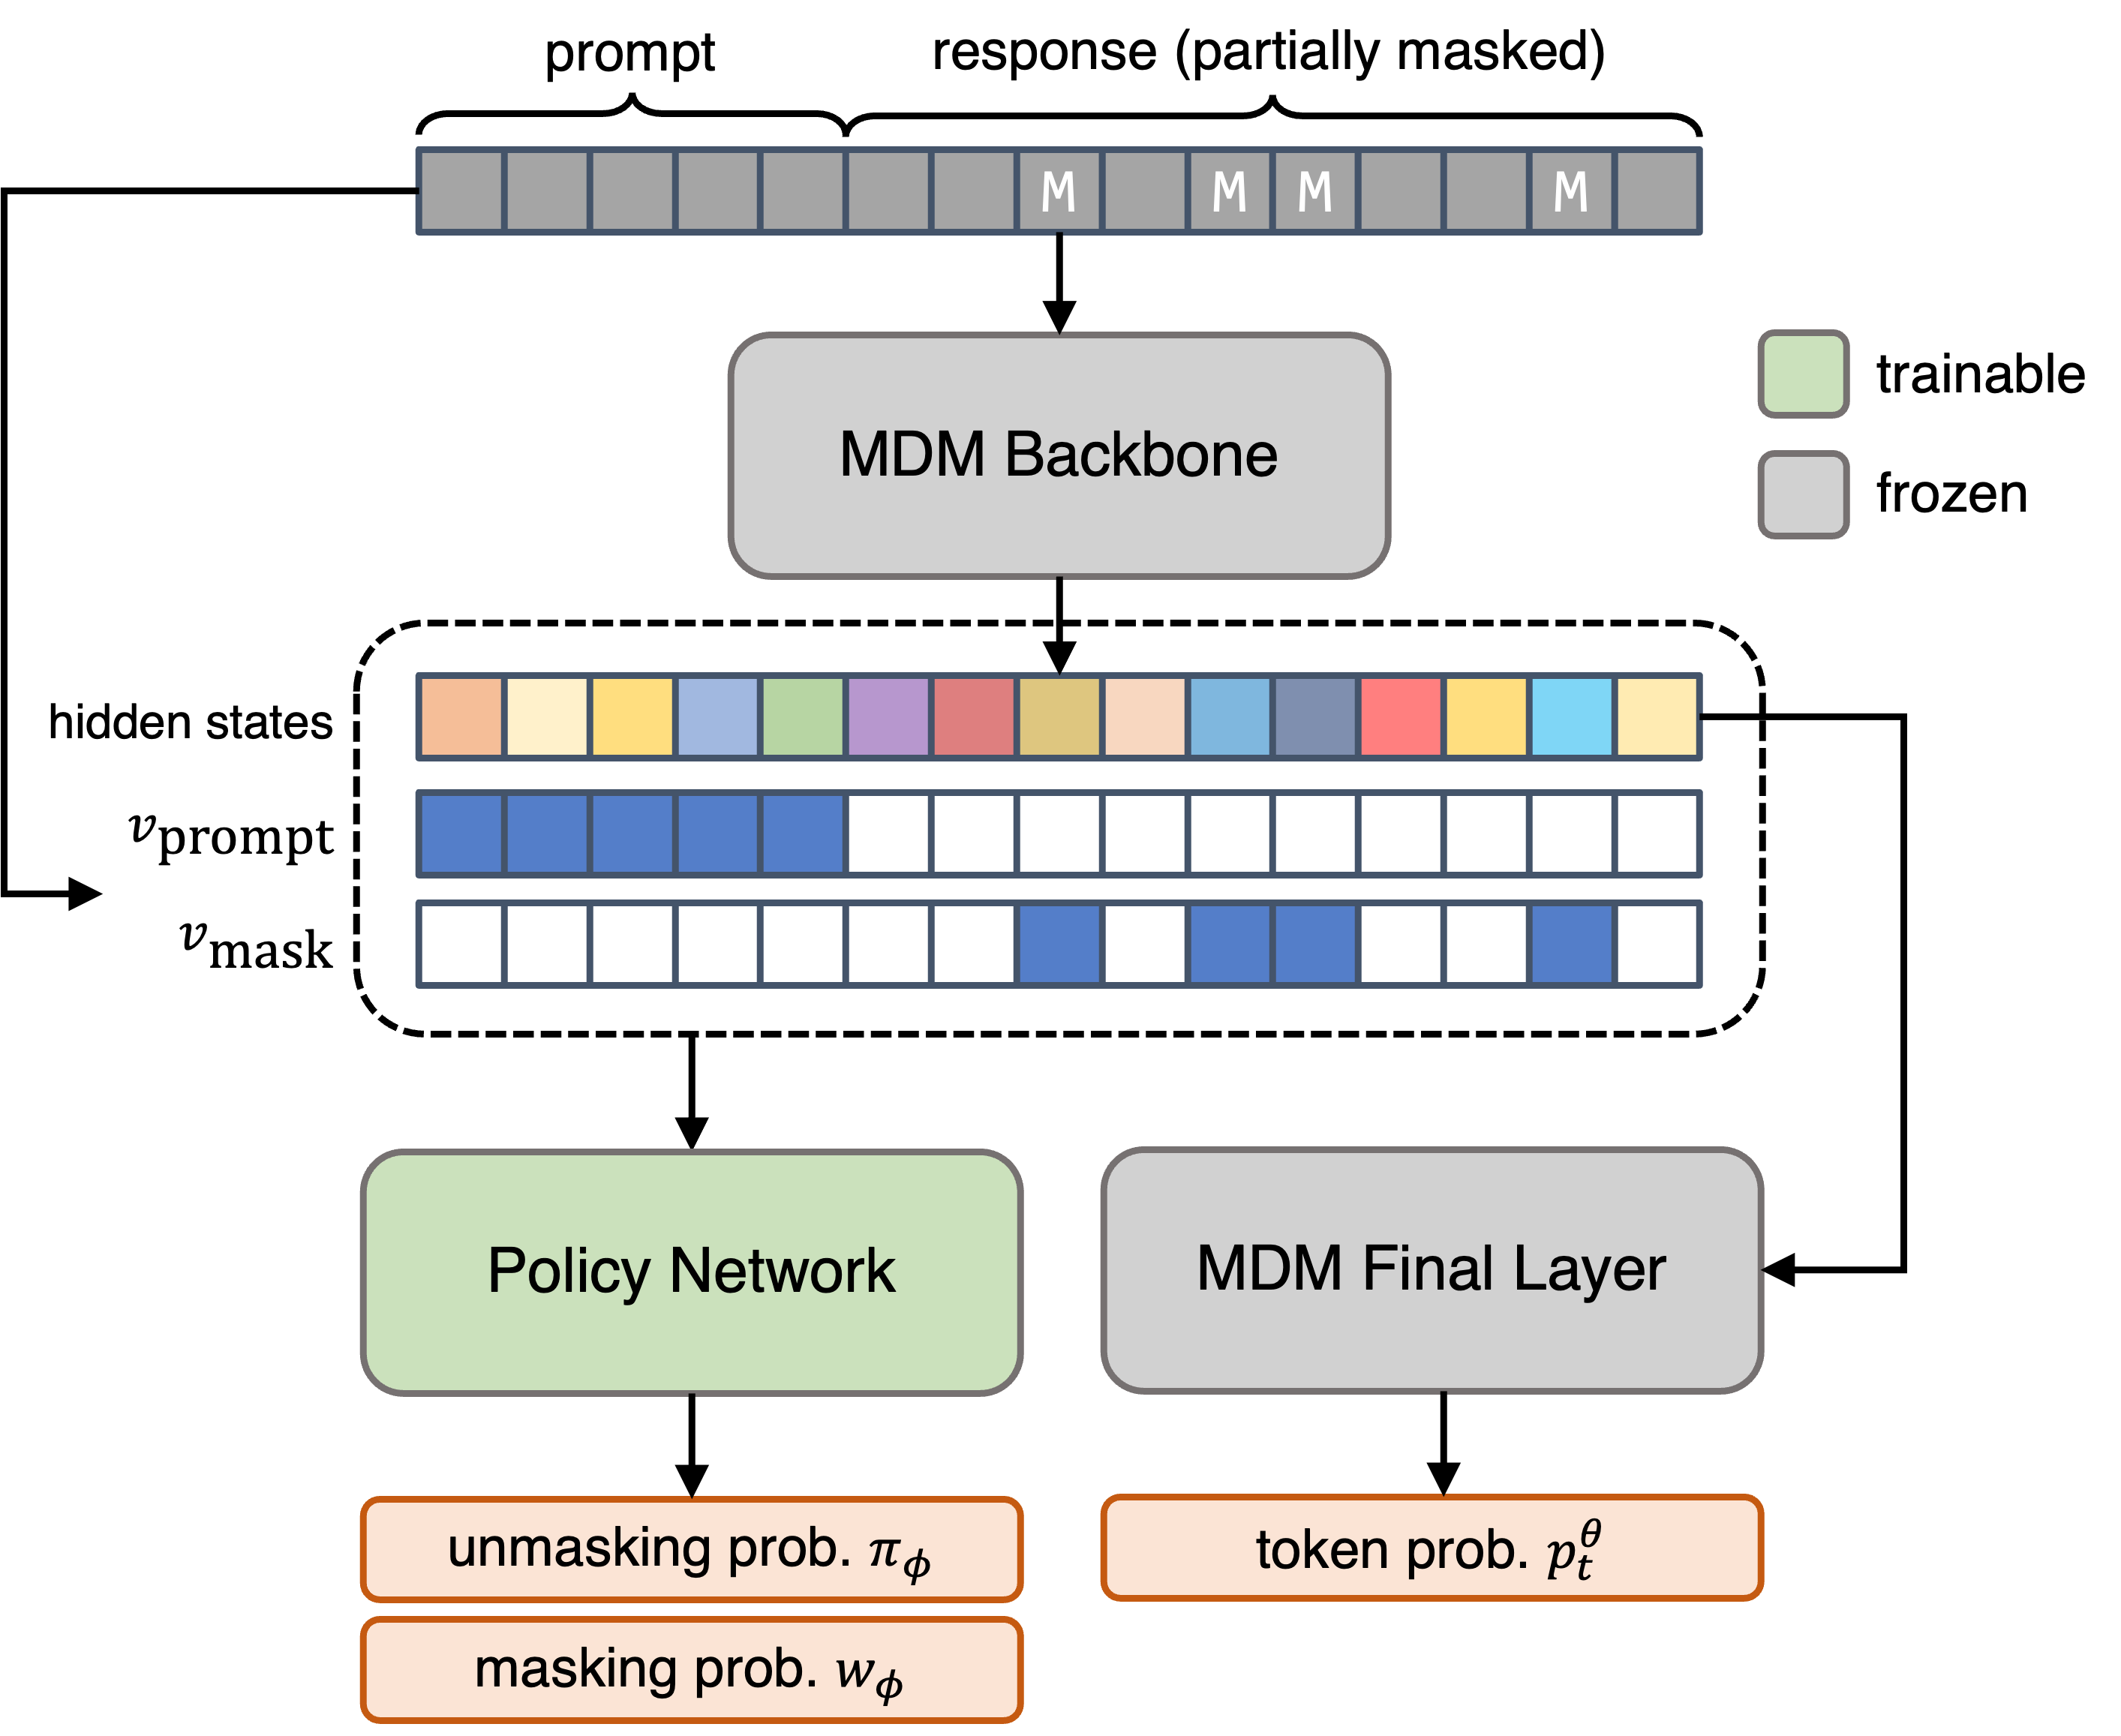
\includegraphics[width=\linewidth]{figs/vlp.png}
    \caption{An illustration of the shared-torso architecture of \alg{} with a trained MDM.}
    \label{fig:vlp}
    \vspace{-1.0em}
\end{wrapfigure}
To represent a policy $\pi_\phi$, we use a neural network that takes current sampling state $\bm x_{k}$ as input, and outputs a probability distribution over the size-$(L/K)$ index sets $\mathcal U_k$ for the next unmasking step. In our implementation, we adopt a shared-torso architecture: the policy network reuses the trained backbone of the MDM and appends an additional lightweight module. This reduces the number of trainable parameters: we pass the MDM's final-layer hidden states $\bm h_k$ to the policy in place of the raw tokens $\bm x_k$. A similar parameterization applies to the distribution $w$.

In our implementation, the additional module is a single-layer Transformer \citep{vaswani2017attention} block with bidirectional multi-head attention and rotary positional embedding \citep{su2023roformerenhancedtransformerrotary}. In addition to the hidden states $\bm h_{k}$, via concatenation, we also input two binary embeddings $\bm v_\text{mask}=(\mathbf1_{x_k^1=\mask},...,\mathbf1_{x_k^L=\mask})\in\{0,1\}^L$ and $\bm v_\text{prompt}=(\mathbf1_{x_k^1\text{ is prompt}},...,\mathbf1_{x_k^L\text{ is prompt}})\in\{0,1\}^L$ to explicitly provide the mask and prompt positions of the sequence. The output is a probability vector $\bm p=(p_1,...,p_L)$ through an application of the softmax function. It models a multinomial distribution over index sets, where each index $i$ is randomly selected to join $\mathcal U_k$ with probability $p_i$. We adopt the multinomial parameterization rather than independent per-position Bernoulli draws (as in, e.g., \citet{chen2025dultra}) since it natively models distributions over fixed-size index sets; in early experiments, an independent-Bernoulli variant collapsed toward unmasking very few tokens per step, since such low-cardinality outcomes have higher joint probability under the model. We illustrate the above design in Figure~\ref{fig:vlp}.

\iffalse
\subsection{Policy Parameterization with Gumbel Trick}
Recall that we constrain our policy to (randomly) output unmasking set of fixed size $N$. To this end, we make use of Gumbel Top-$N$ trick for efficient sampling and computation. Specifically, given policy network's output $\bm p=(p_1,p_2,...,p_L)\in\Delta([L])$, we randomly decide an index set $\mathcal U$ with $|\mathcal U|=N$ by sampling $\bm g\sim\mathrm{Gumbel(0,1)}$ and then pick the top-$N$ indices
\begin{align*}
    \mathcal U=\mathrm{top}_N(\log\bm p +\bm g).
\end{align*}
By this Gumbel sampling trick, the policy indeed assigns $\mathcal U$ with probability
\begin{align*}
    \pi(\mathcal U)&=\Pr\left(\min_{i\in\mathcal U}\log p_i+g_i>\max_{j\neq\mathcal U}\log  p_j+g_j\right)\\
    &=\int_0^\infty \prod_{i\in\mathcal U} p_ie^{-p_it}\prod_{j\notin\mathcal U}(1-e^{-p_jt})dt\\
    &=\int_0^1 \prod_{i\in\mathcal U} p_is^{p_i}\prod_{j\notin\mathcal U}(1-s^{p_j})\frac{1}{s}ds.
\end{align*}
Therefore we can compute an unbiased estimate for $\pi(\mathcal U)$.
\fi


\subsection{Training and Inference}
We summarize training and inference of \alg{} in Algorithm~\ref{alg:train} and~\ref{alg:inf}, respectively. In general, at each training iteration we draw a data sample $\bm x_0\sim q_0$, sample a masking trajectory from $w_\phi$, and compute the corresponding unmasking loss using $\pi_\phi$. Since $\phi$ also appears in the sampling of the masking trajectory from $w_\phi$, the stochastic gradients $\nabla_\phi s^{(i)}$ must be corrected via REINFORCE \citep{wang2025learningorder} to obtain an unbiased estimate $g_\text{REINFORCE}=\nabla_\phi s^{(i)}+(s^{(i)}-s)\nabla_\phi\log w^{(i)}$. While REINFORCE is known to have high gradient variance \citep{shi2022gradient}, we retain this estimator to maintain methodological compatibility with \citet{wang2025learningorder}, whose framework our work extends to multi-token unmasking. Lower-variance alternatives are left to future work. At the inference stage, we directly use the trained policy to sample an unmasking index set and apply the trained MDM to predict tokens.


\begin{algorithm}[tb]
  \caption{\alg{} Training}
  \label{alg:train}
  \begin{algorithmic}[1]
    \Input Initialization $\phi$, trained MDM $p^\theta_t$, dataset $\mathcal D$, batch size $B$, total sampling steps $K$, learning rate $\eta$, regularization strength $\lambda$
    \Output Trained policy $\pi_\phi$
    \Repeat
      \State Sample data batch $\{\bm x_0^{(i)}\}_{i=1}^B \sim \mathcal D$
      \For{$i=1,\ldots,B$}
        \State Sample $\mathcal U^{(i)} \sim w_\phi(\cdot \mid \bm x_0^{(i)})$
        \State Construct $\bm x_1^{(i)},\ldots,\bm x_K^{(i)}$ according to $\mathcal U^{(i)}$
        \State $w^{(i)} \gets w_\phi(\mathcal U^{(i)} \mid \bm x_0^{(i)})$
        \State $p^{(i)} \gets \prod_{k=1}^K
        p^\theta_{t_k}(\bm x_{k-1}^{(i)} \mid \bm x_k^{(i)})
        \pi_\phi(\mathcal U_{k}^{(i)} \mid \bm x_k^{(i)})$
        \State $r^{(i)} \gets
        \sum_{k=1}^K
        \mathrm{KL}\!\left(
        \pi_\phi(\cdot \mid \bm x_k^{(i)})
        \,\|\, 
        \pi_{\mathrm{ref}}(\cdot \mid \bm x_k^{(i)})
        \right)+
        \mathrm{KL}\!\left(
        w_\phi(\cdot \mid \bm x_0^{(i)})
        \,\|\,
        w_{\mathrm{ref}}(\cdot \mid \bm x_0^{(i)})
        \right)$
        \State $s^{(i)} \gets \log w^{(i)} - \log p^{(i)} + \lambda r^{(i)}$
      \EndFor
      \State $s \gets \frac{1}{B}\sum_{i=1}^B s^{(i)}$
      \State $g_{\text{REINFORCE}} \gets
      \frac{1}{B}\sum_{i=1}^B
      \left[
      \nabla_\phi s^{(i)}
      +
      \left(s^{(i)} - s\right)
      \nabla_\phi \log w^{(i)}
      \right]$
      \State $\phi \gets \phi - \eta\, g_{\text{REINFORCE}}$
    \Until{converged}
  \end{algorithmic}
\end{algorithm}

\begin{algorithm}[tb]
  \caption{\alg{} Inference}
  \label{alg:inf}
  \begin{algorithmic}[1]
    \Input Policy $\pi_\phi$, trained MDM $p^\theta_t$, total sampling steps $K$, sequence length $L$
    \Output Generated sample $\bm x_0$
    \State $\bm x_K \gets (\mask{}, \mask{}, \ldots, \mask{})$
    \For{$k=K,\ldots,1$}
      \State Sample $\mathcal U_{k} \sim \pi_\phi(\cdot \mid \bm x_k)$
      \State Sample candidate tokens $\hat{\bm x}_{k-1} \sim p_{t_k}^\theta(\cdot \mid \bm x_k)$
      \State Construct $\bm x_{k-1}$ elementwise by
      \[
        x_{k-1}^i
        \gets
        \hat{x}_{k-1}^i \mathbf{1}_{i \in \mathcal U_k}
        +
        x_k^i \mathbf{1}_{i \notin \mathcal U_k}
      \]
    \EndFor
    \State \Return $\bm x_0$
  \end{algorithmic}
\end{algorithm}
\section{Further Details on Experiments}\label{sec:experiment-appendix}
\subsection{Optimality Analysis}
\subsubsection{Synthetic Experiments}\label{subsec:synthetic}

We use a small synthetic setting to visualize the likelihood-optimization landscape for unmasking policies. The sequence length is set to $L=3$, the vocabulary size to $V=10$, and the number of unmasked positions selected at each step to $N=2$. We generate a product data distribution by sampling token logits independently and applying position-dependent temperatures $(0.1,0.5,2.0)$, followed by a softmax normalization. This creates positions with different uncertainty levels.

For each policy, we evaluate the objective exactly by enumerating all clean sequences in $[V]^L$ and all possible $N$-hot unmasking masks. Since positions are sampled without replacement, the probability of each unordered mask is computed exactly by dynamic programming over all possible sampling orders. We compare uniform sampling, greedy confidence sampling, and randomized confidence sampling. The confidence scores are based on negative entropy, top-token probability, and top-2 probability margin. For randomized confidence policies, we apply a softmax over the scores with various temperatures $T \in \{0.1,0.2,\ldots,2.0,3,5,8,10\}$.

To find an approximate optimum, we enumerate a regular grid over the policy simplex and evaluate the exact objective at each grid point. Each policy is mapped to its induced distribution over the 3 possible 2-position masks, yielding a visualization on the mask-probability simplex. We then plot the objective landscape, the optimizer, the uniform and greedy confidence methods, and a continuum of random confidence methods as the temperature $T$ varies. In Figure~\ref{fig:policy-simplex-seed}, we provide more landscape visualization plots under different random seeds for the synthetic data generation.

\begin{figure}[h]
    \centering
    \begin{subfigure}[h]{0.48\linewidth}
        \centering
        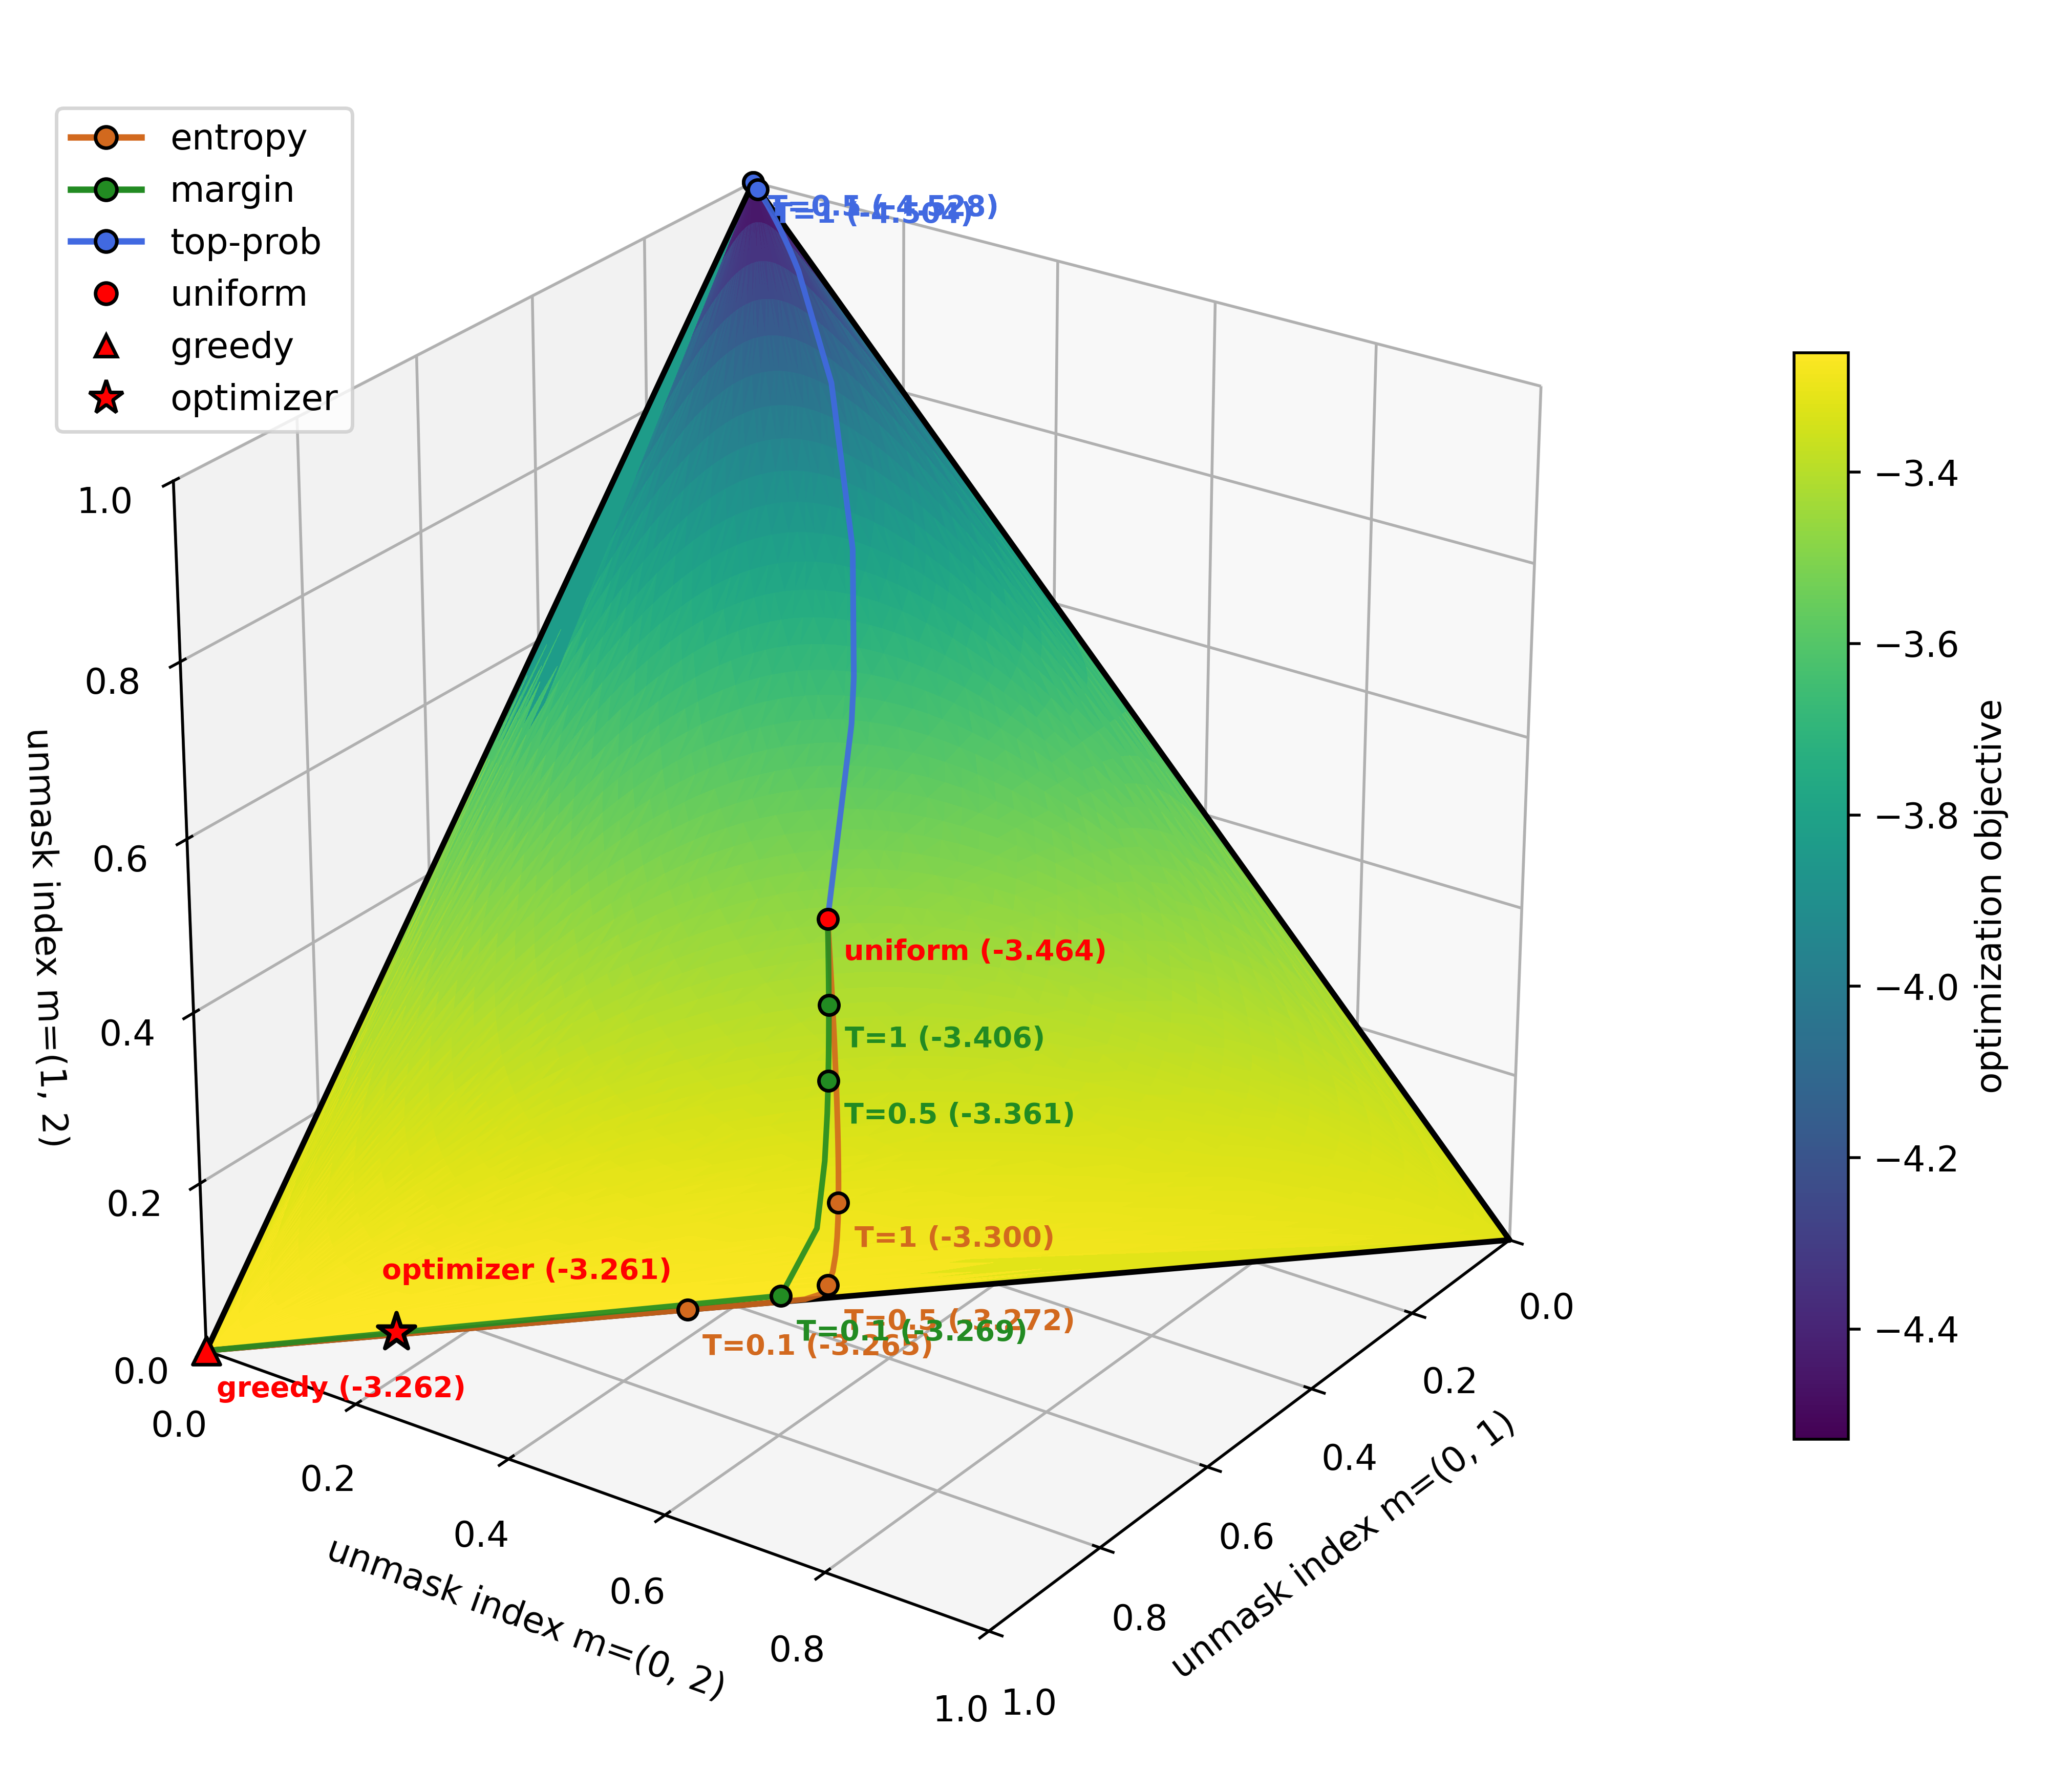
\includegraphics[width=\linewidth]{figs/policy_simplex_seed_6.png}
    \end{subfigure}
    \hfill
    \begin{subfigure}[h]{0.48\linewidth}
        \centering
        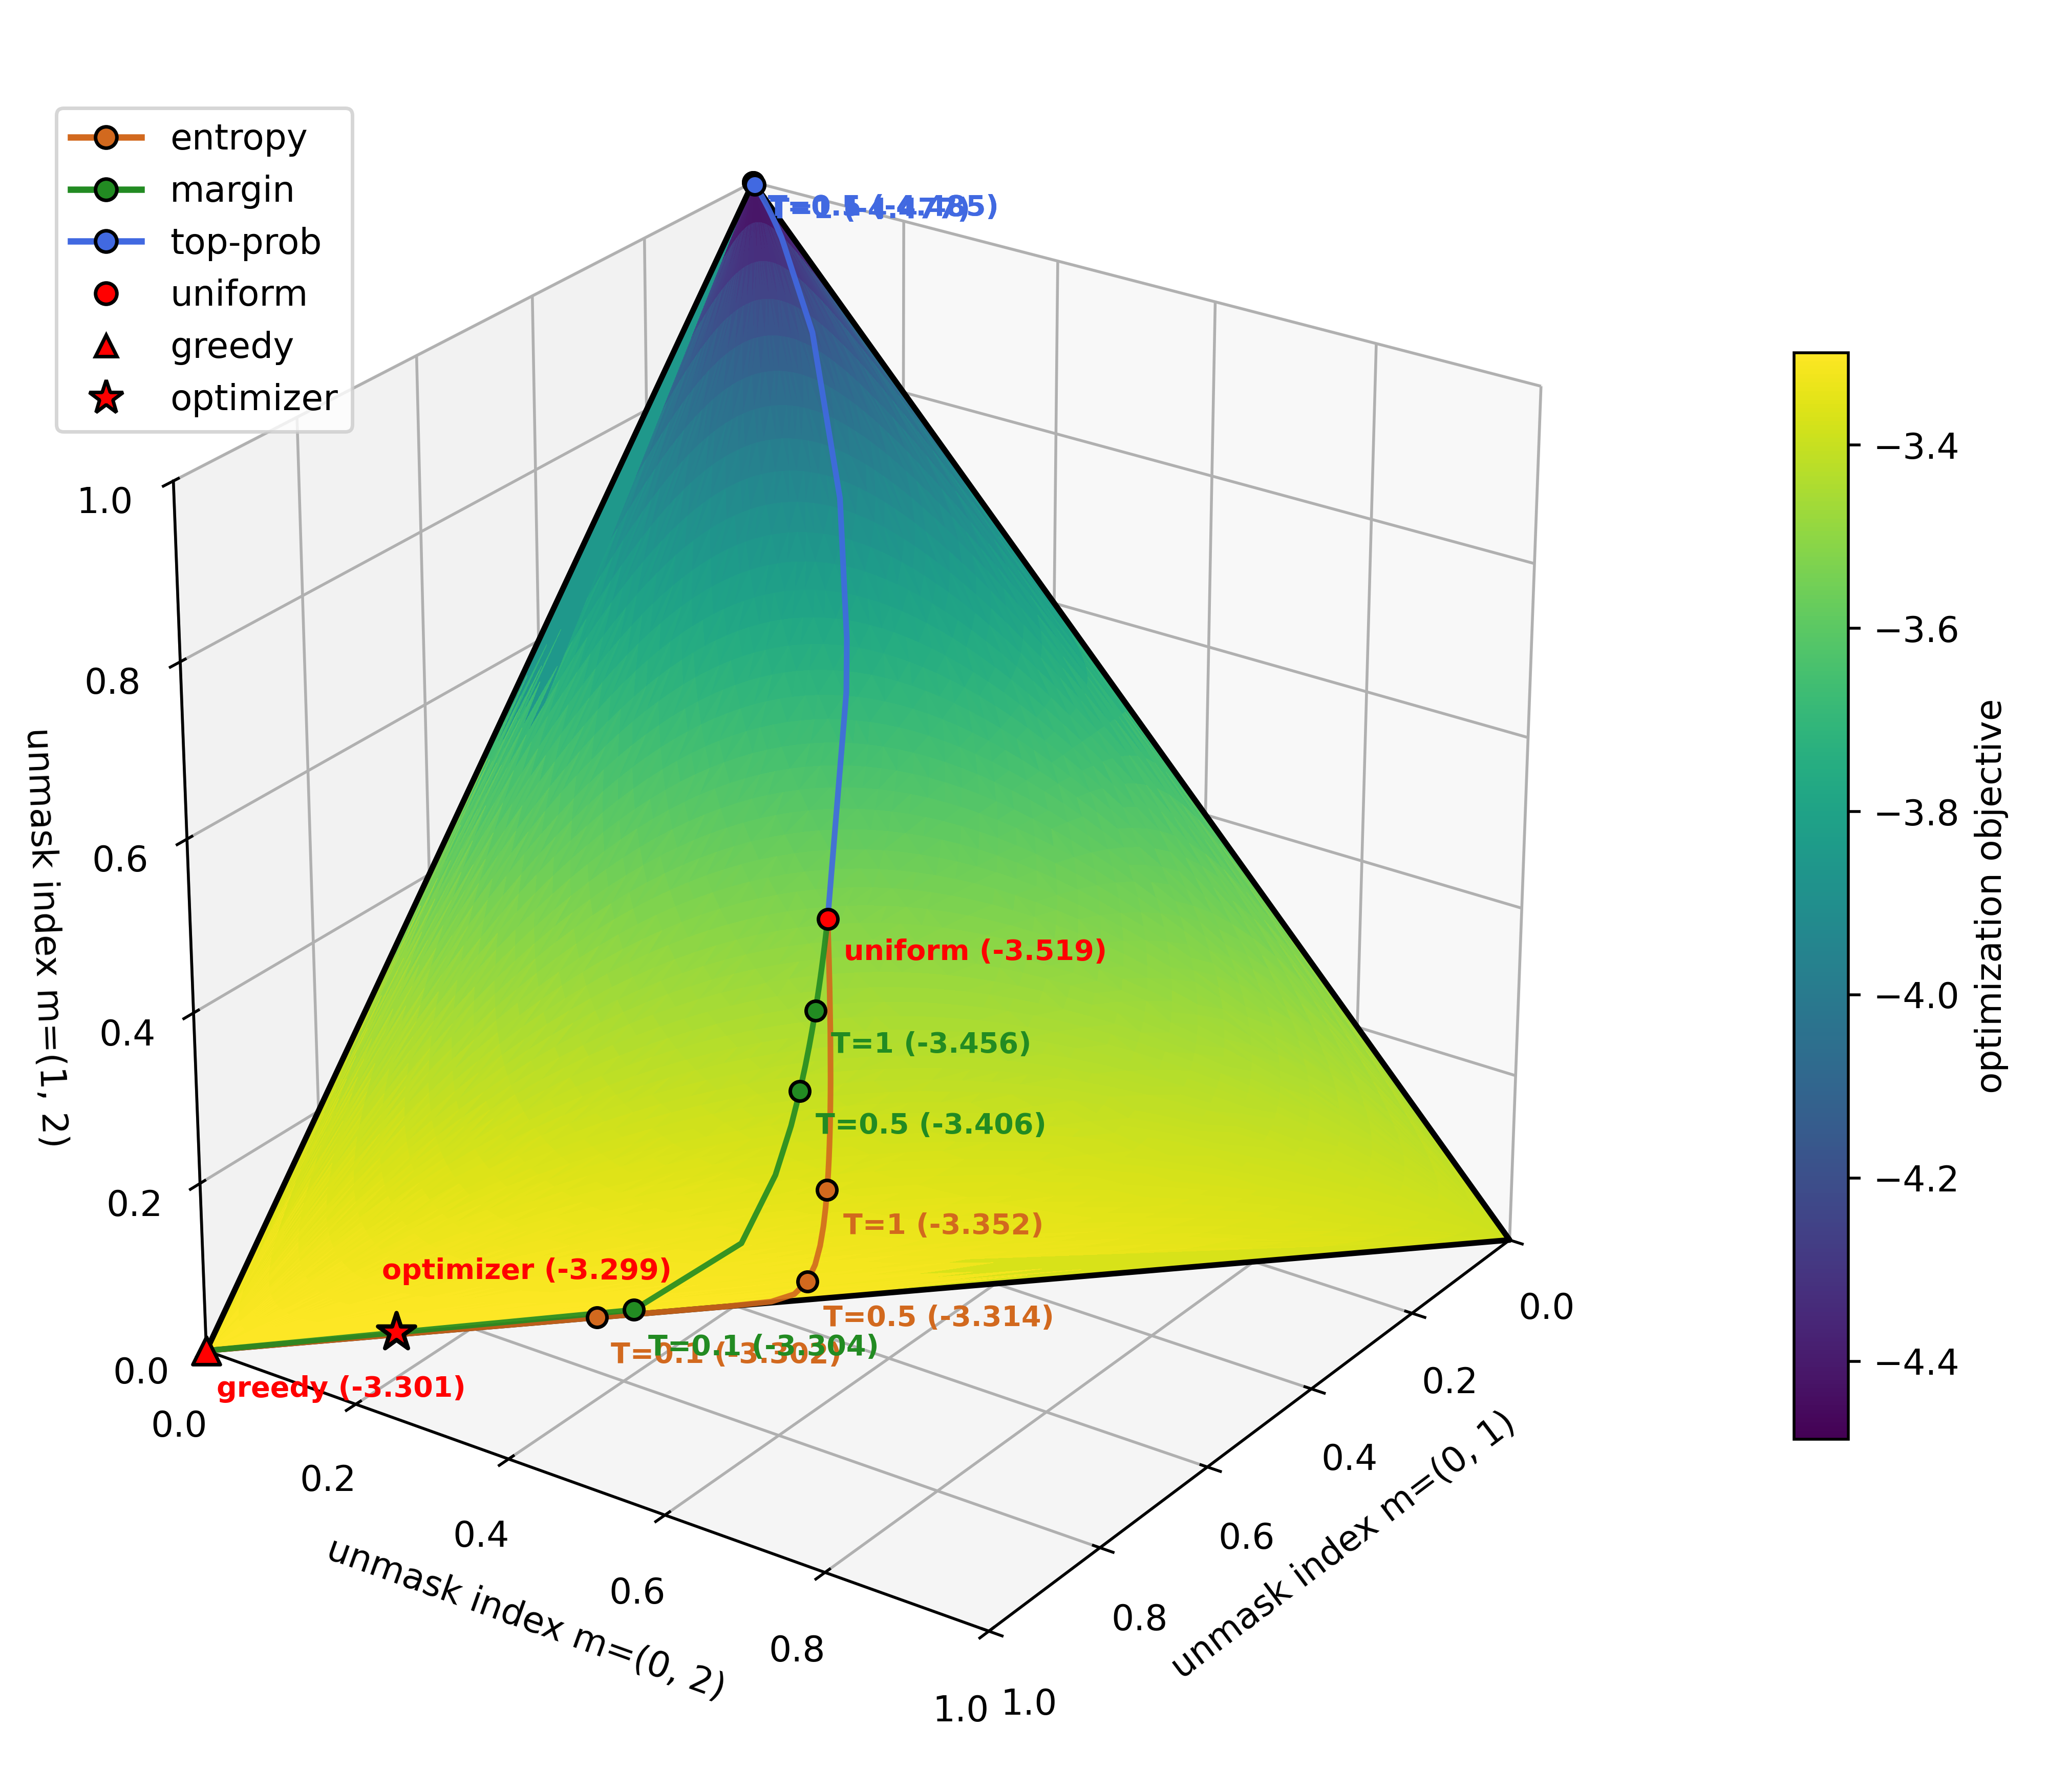
\includegraphics[width=\linewidth]{figs/policy_simplex_seed_8.png}
    \end{subfigure}
    \\
    \begin{subfigure}[h]{0.48\linewidth}
        \centering
        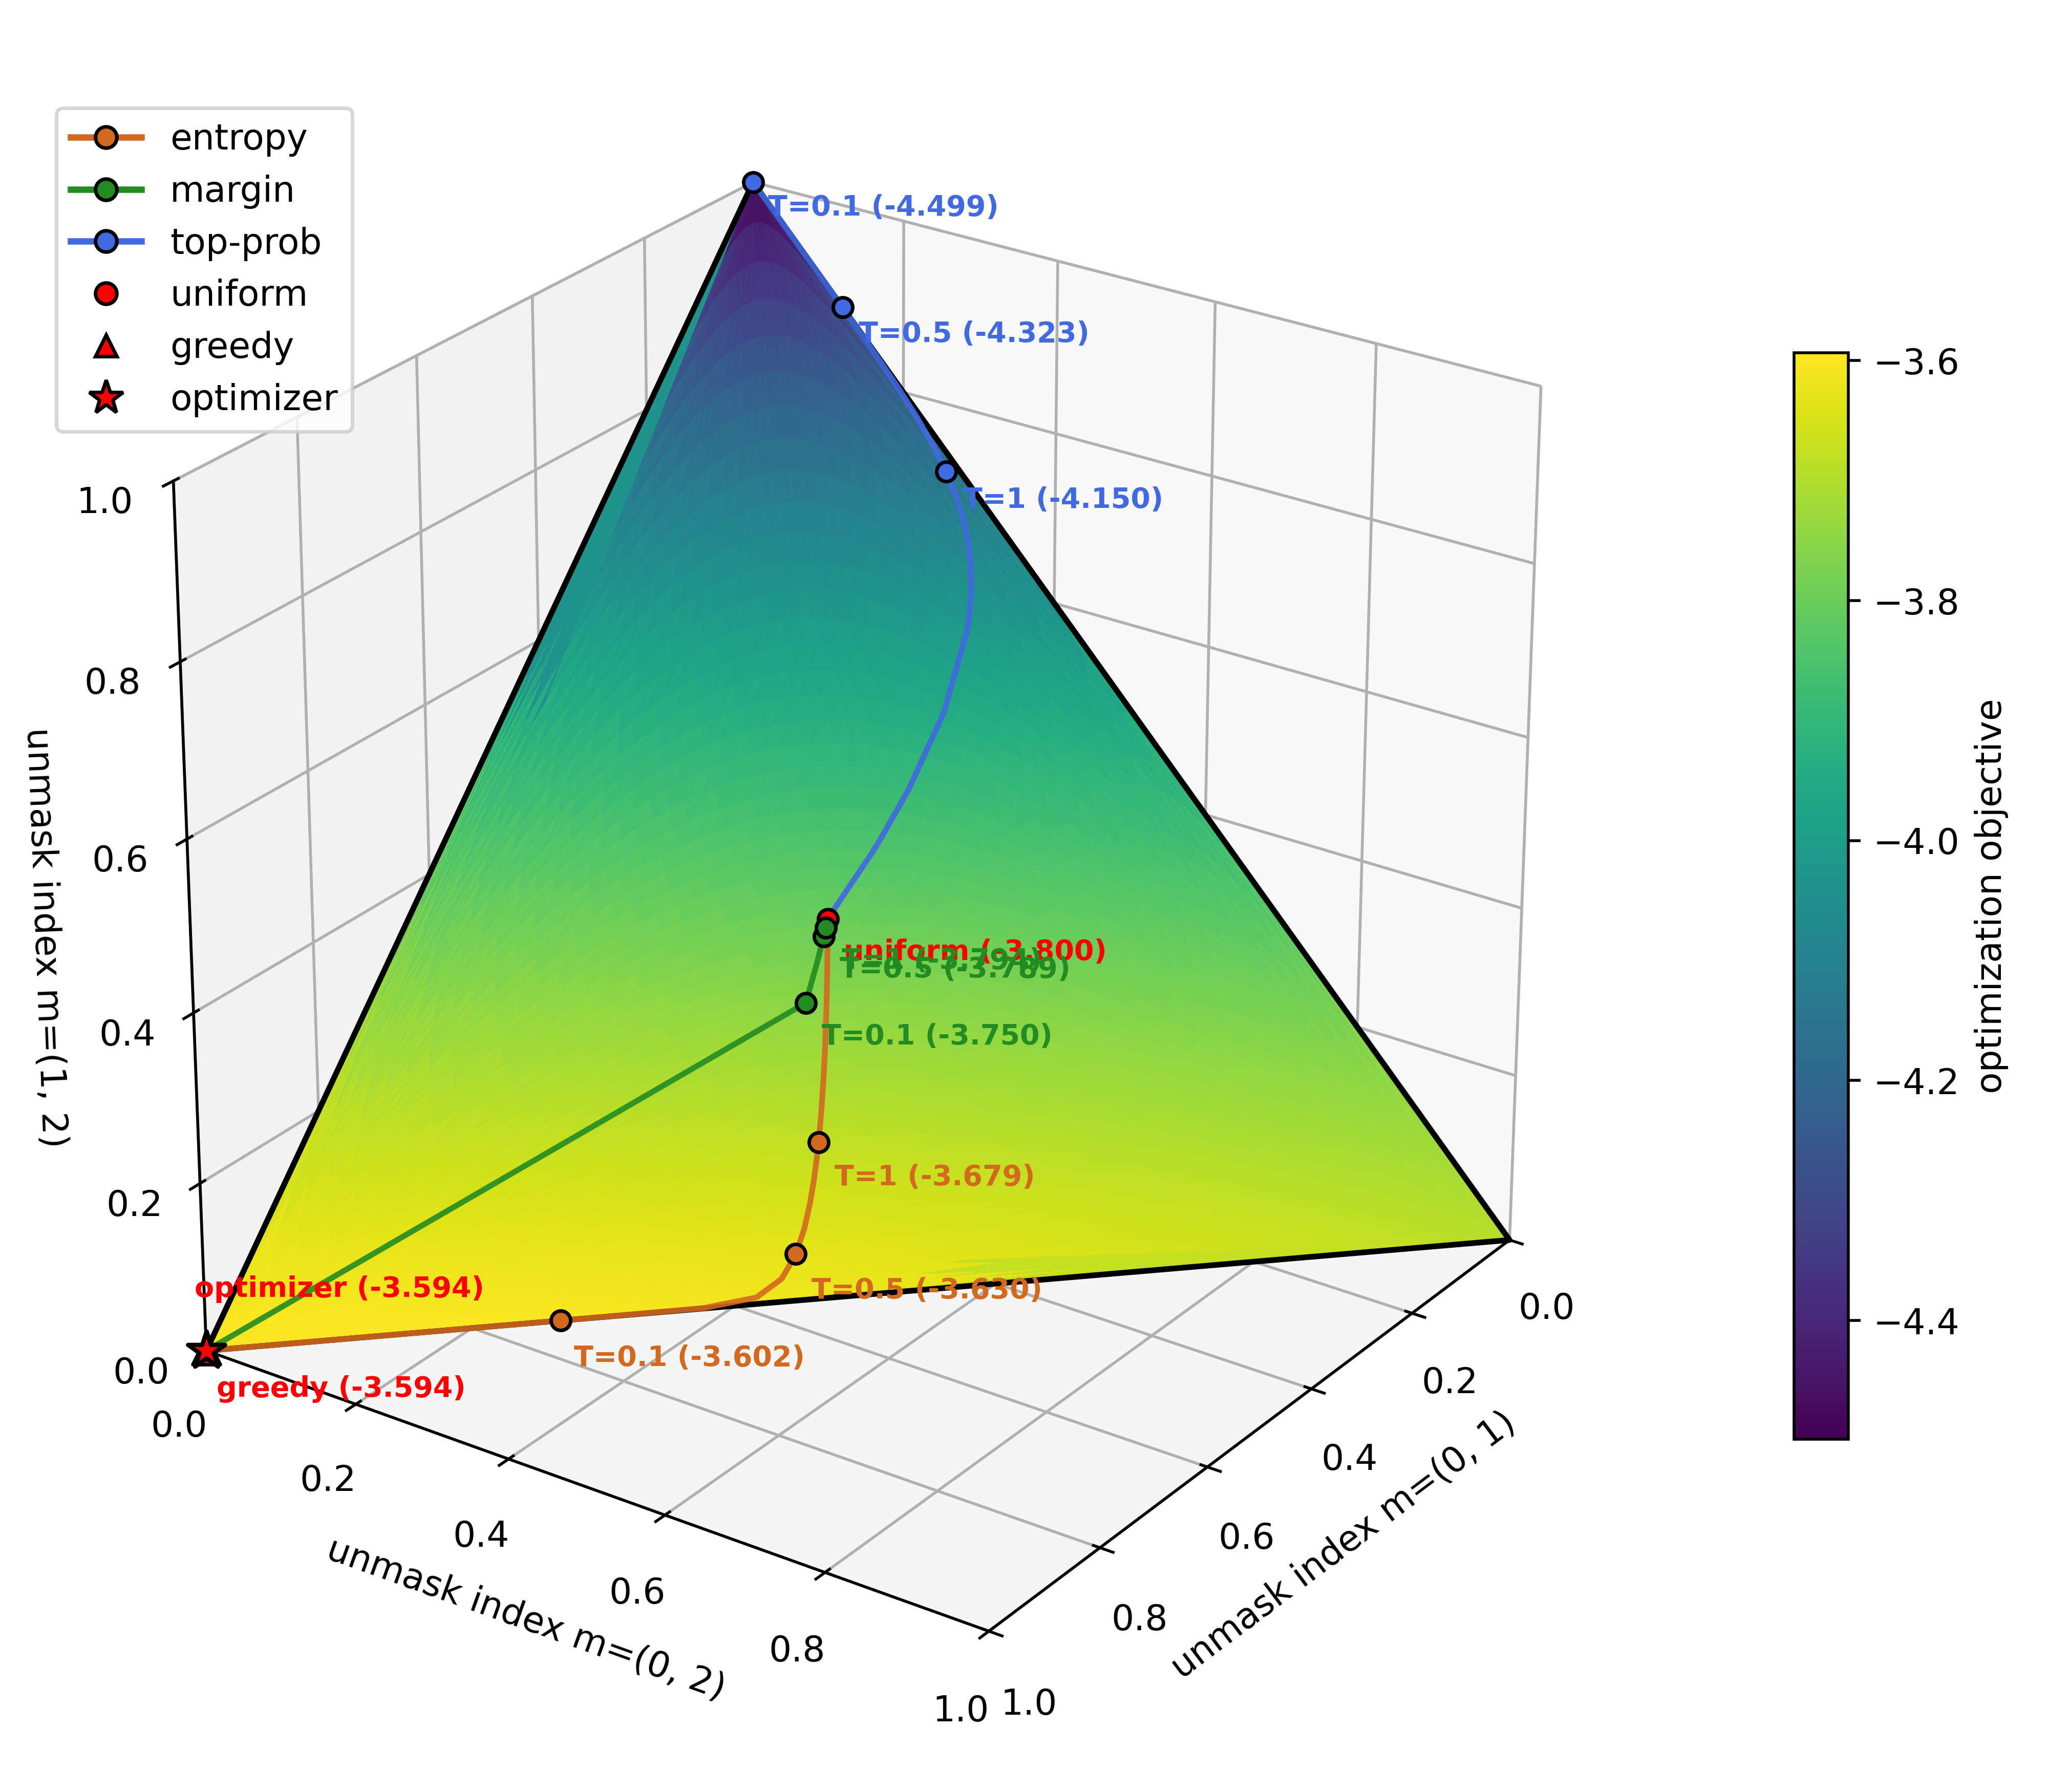
\includegraphics[width=\linewidth]{figs/policy_simplex_seed_10.png}
    \end{subfigure}
    \hfill
    \begin{subfigure}[h]{0.48\linewidth}
        \centering
        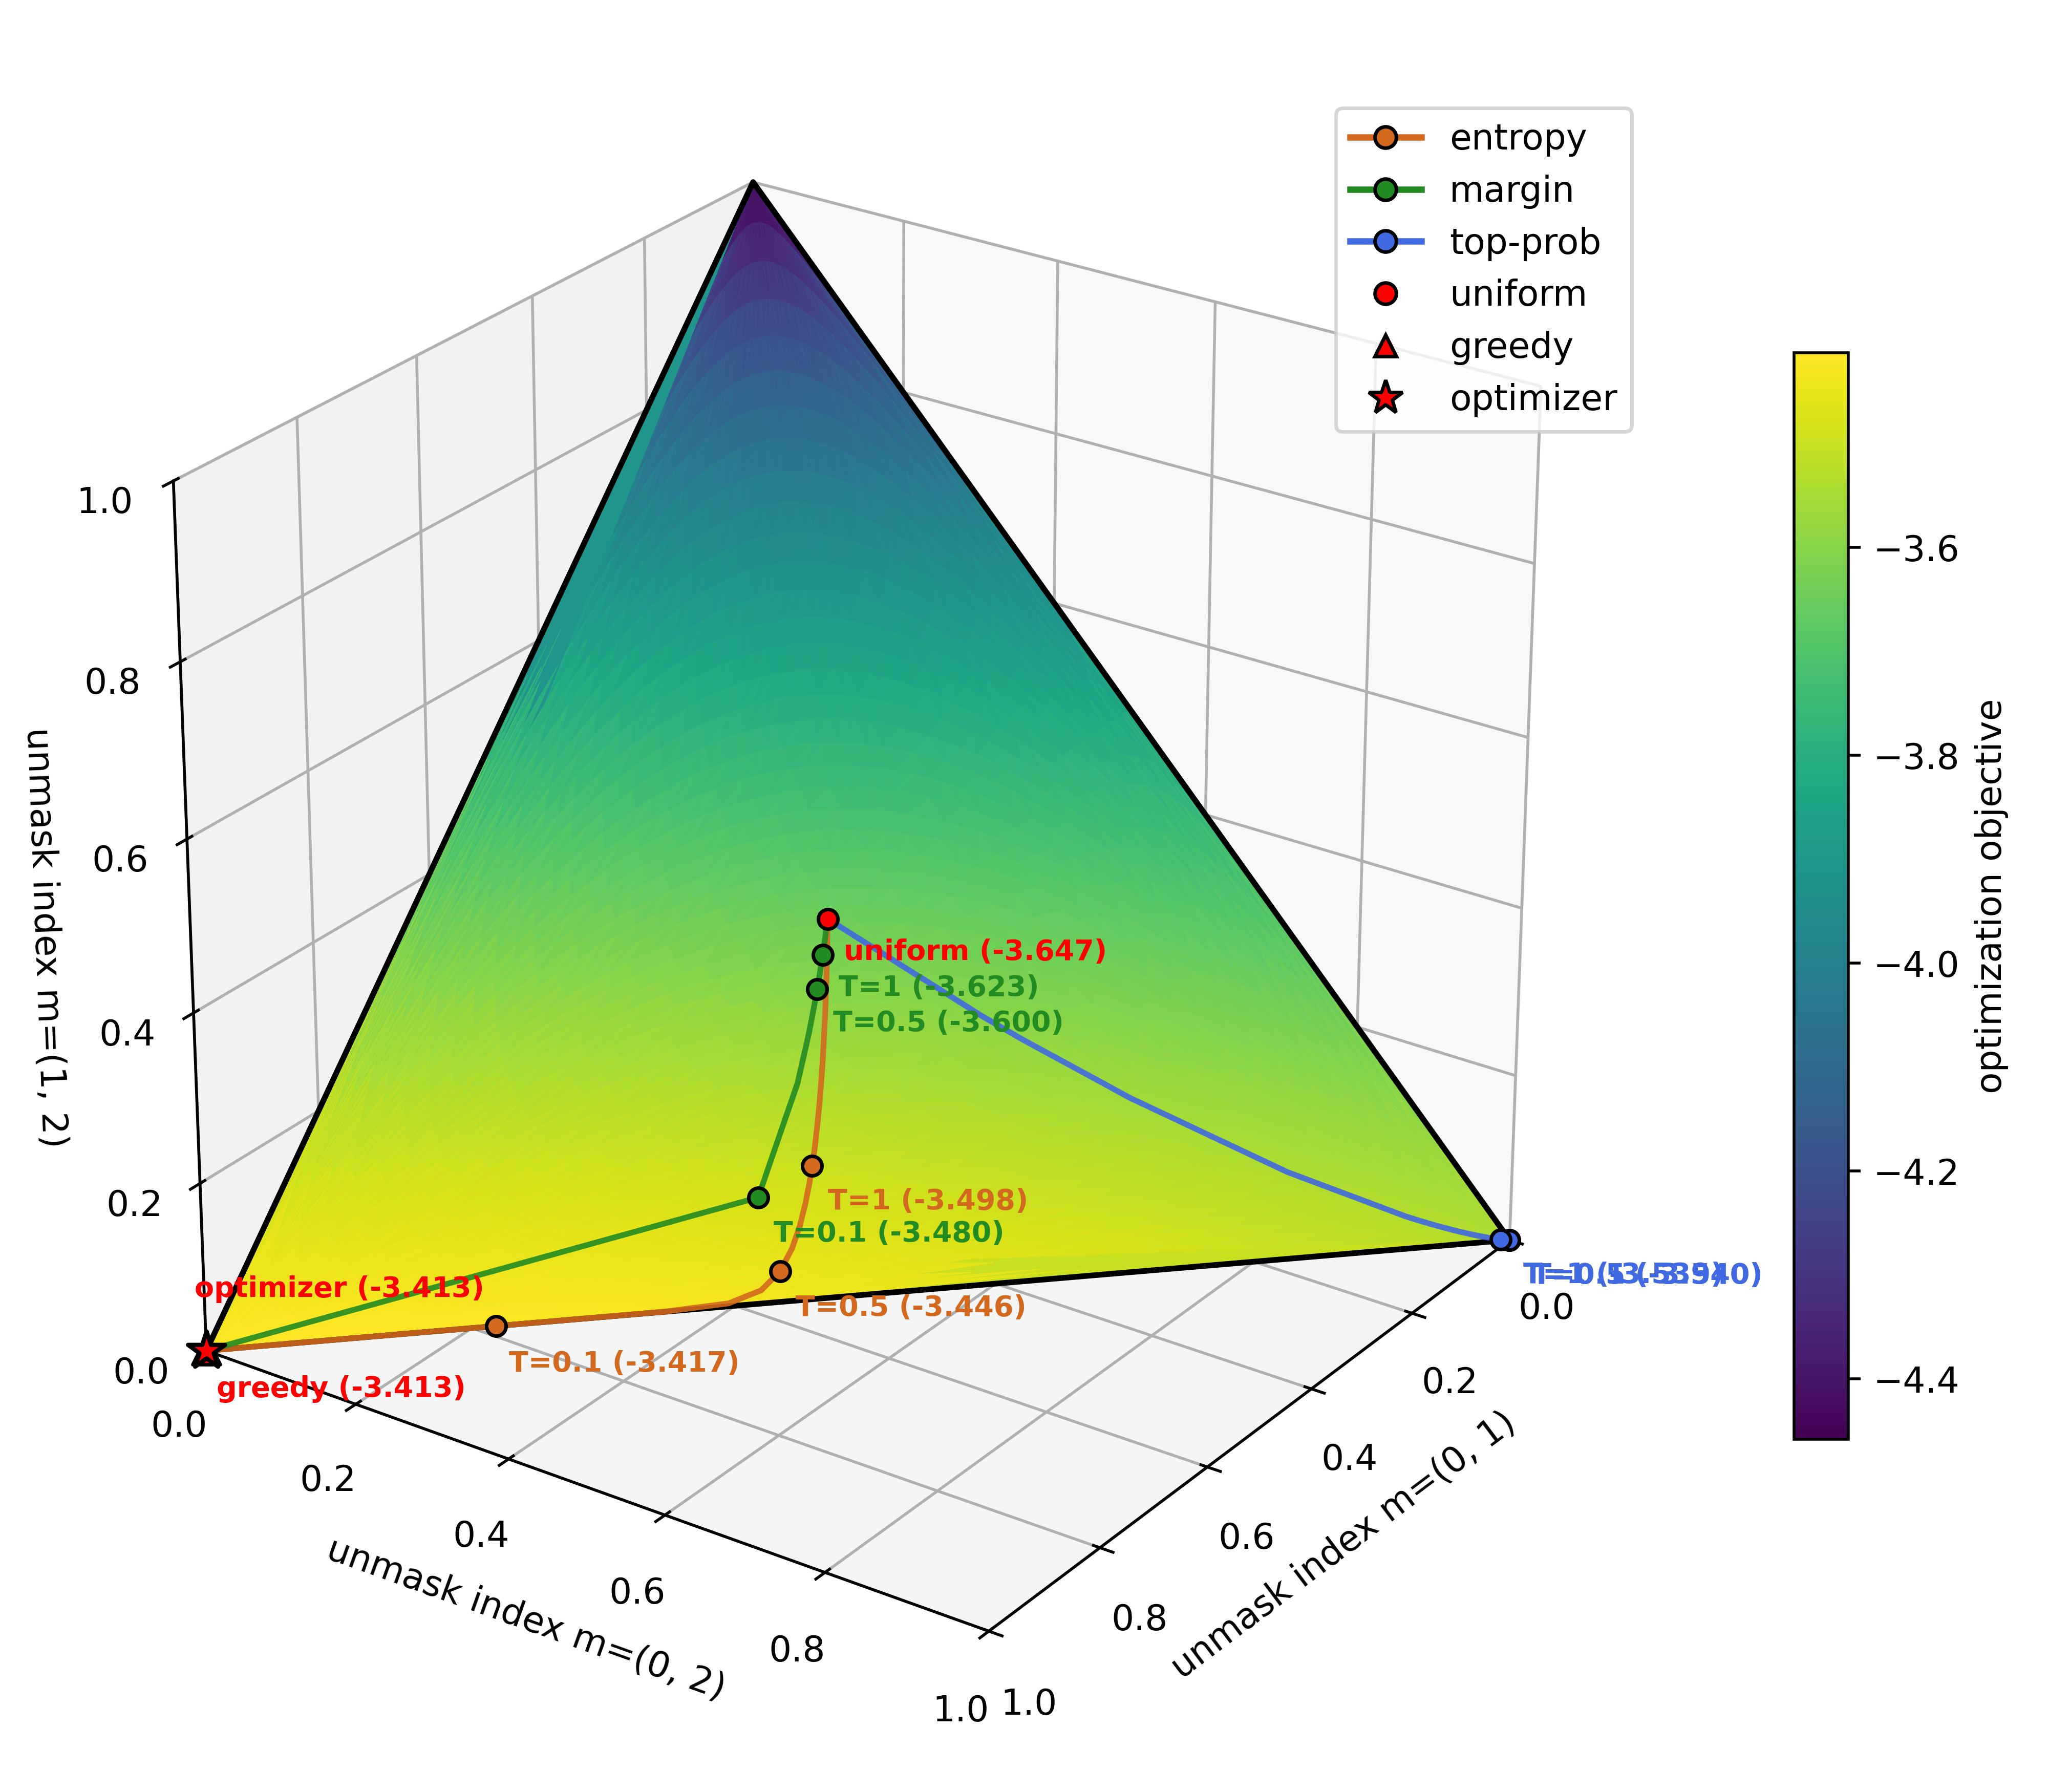
\includegraphics[width=\linewidth]{figs/policy_simplex_seed_12.png}
    \end{subfigure}
    \caption{Policy simplex and different unmasking strategies under various choices of data-generating seed in the synthetic data.}
    \label{fig:policy-simplex-seed}
\end{figure}

\subsubsection{Text Generation Experiments}\label{subsec:radd-gen-exp}

We evaluate the objective value induced by different unmasking strategies during diffusion-based text generation. 
Samples are generated using the pretrained RADD model \citep{ou2024your}. The generation length is fixed to 1024 tokens with batch size 4, and each experiment is repeated over 100 independent sampling runs. 
We vary the number of sampling steps \(N \in \{128,256,512,1024\}\). 
At each sampling step \(i\), the sampler unmasks \(1024/N\) token positions. We compare three strategies: uniform unmasking, greedy confidence based on top-2 probability margin, and its randomized version.

For each run and sampling step, we estimate the objective value \eqref{eq:trainable_confidence} using Monte Carlo approximation. 
Given the model conditional token distribution at the current partially masked sequence, we sample complete token proposals and random unmasking subsets. 
The objective is estimated from the log probability of selecting the subset together with the conditional token likelihood, with a combinatorial correction for the number of possible subsets. 
In the implementation, we use 10 Monte Carlo token samples and 10 sampled unmasking subsets per step. 
For the greedy case, the objective is computed using the top selected negative-entropy terms. 

For each \(N\), we aggregate the objective values across up to 100 runs for each strategy in Figure~\ref{fig:radd-obj-all-step}. Faint curves display the raw per-run objective trajectories, while solid curves show the mean objective value at each sampling step.

\begin{figure}[h]
    \centering
    \begin{subfigure}[h]{0.48\linewidth}
        \centering
        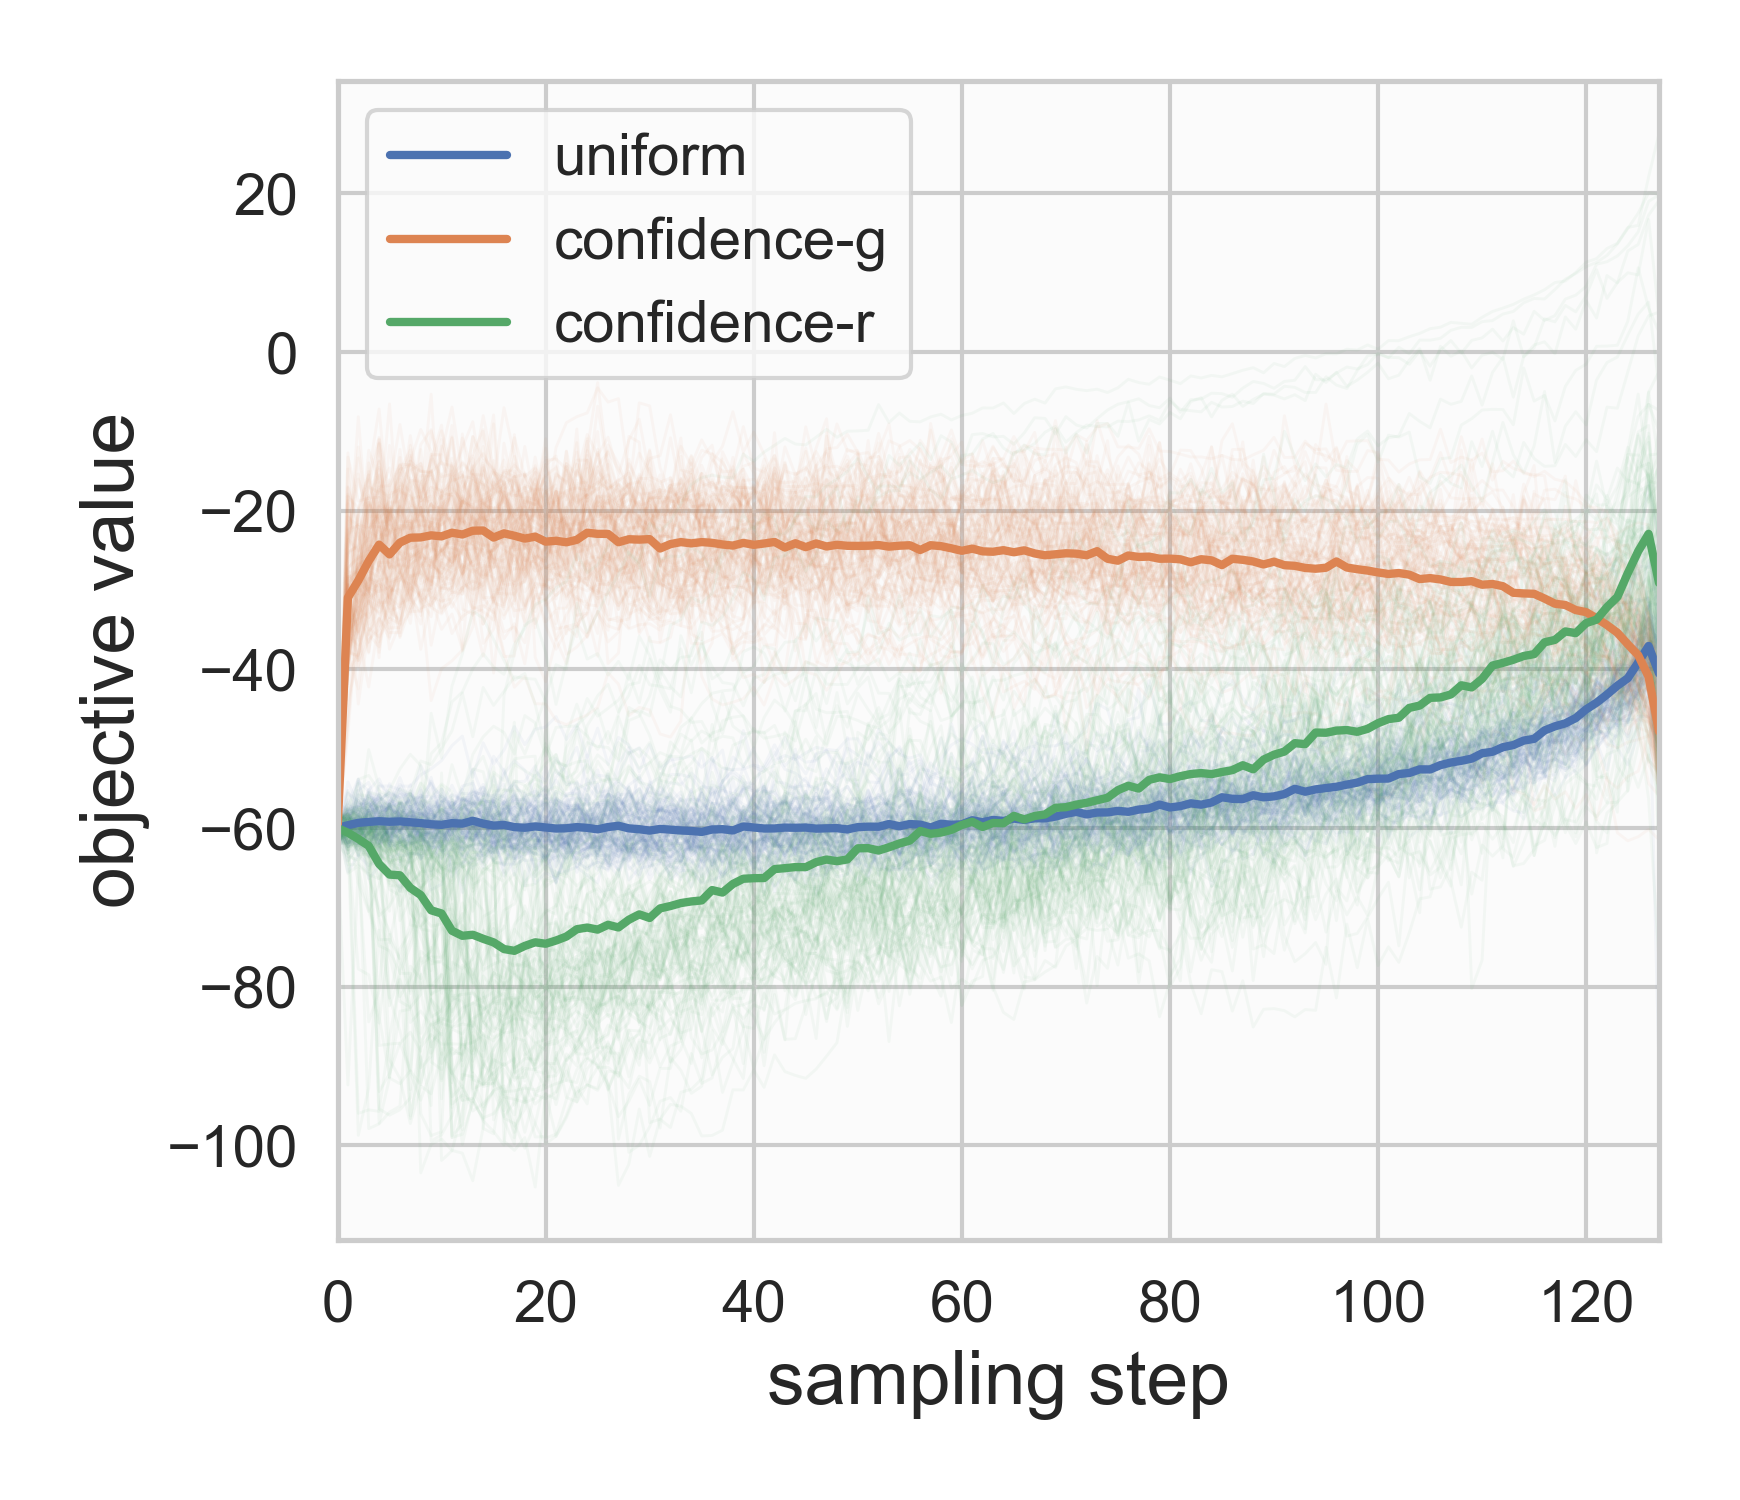
\includegraphics[width=\linewidth]{figs/objective_steps_128.png}
        \caption{128 steps}
    \end{subfigure}
    \hfill
    \begin{subfigure}[h]{0.48\linewidth}
        \centering
        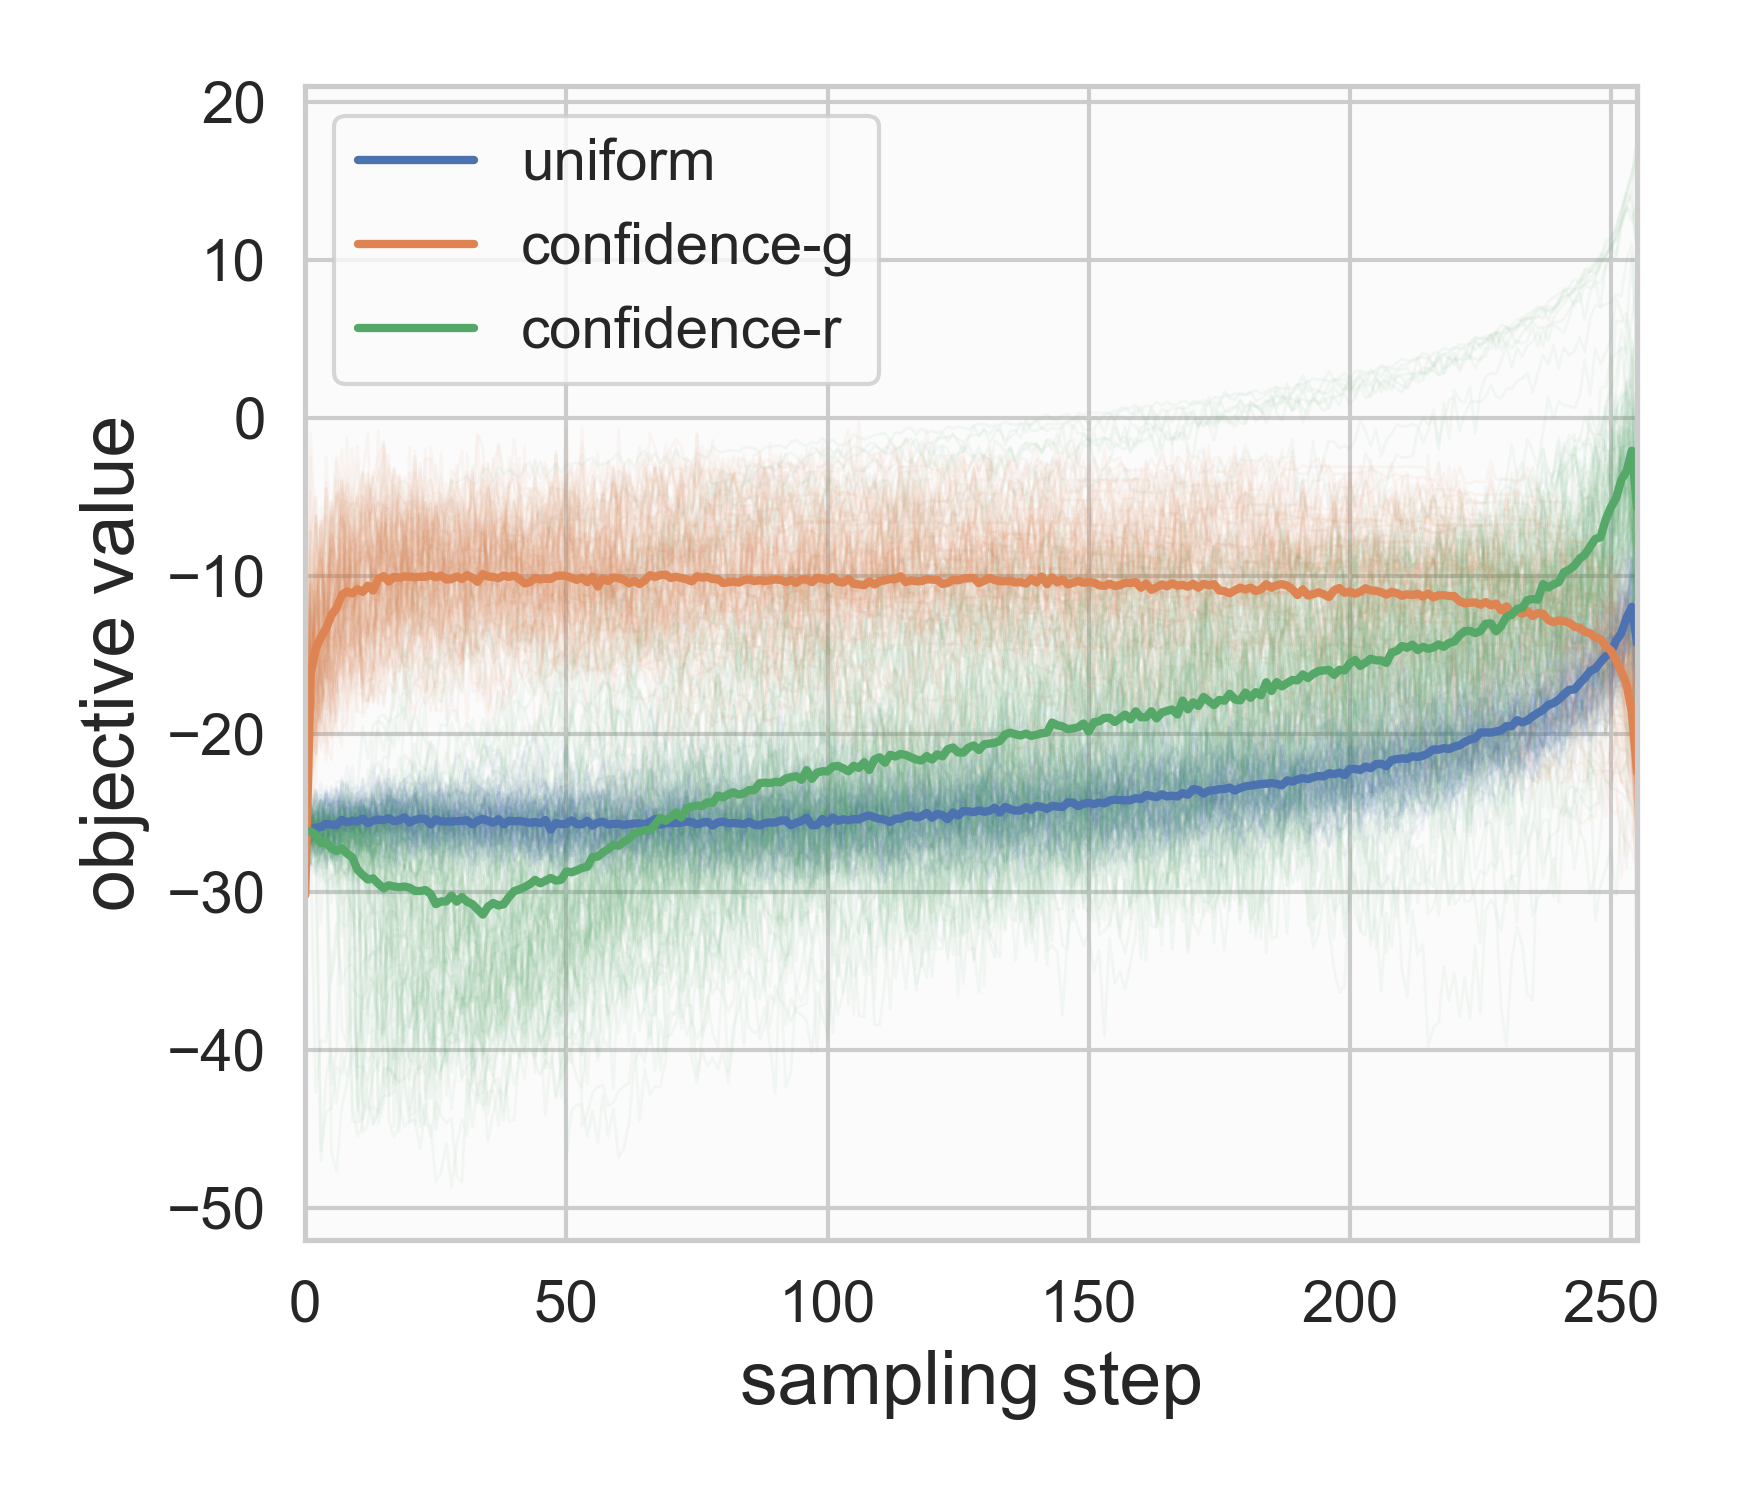
\includegraphics[width=\linewidth]{figs/objective_steps_256.png}
        \caption{256 steps}
    \end{subfigure}
    \\
    \begin{subfigure}[h]{0.48\linewidth}
        \centering
        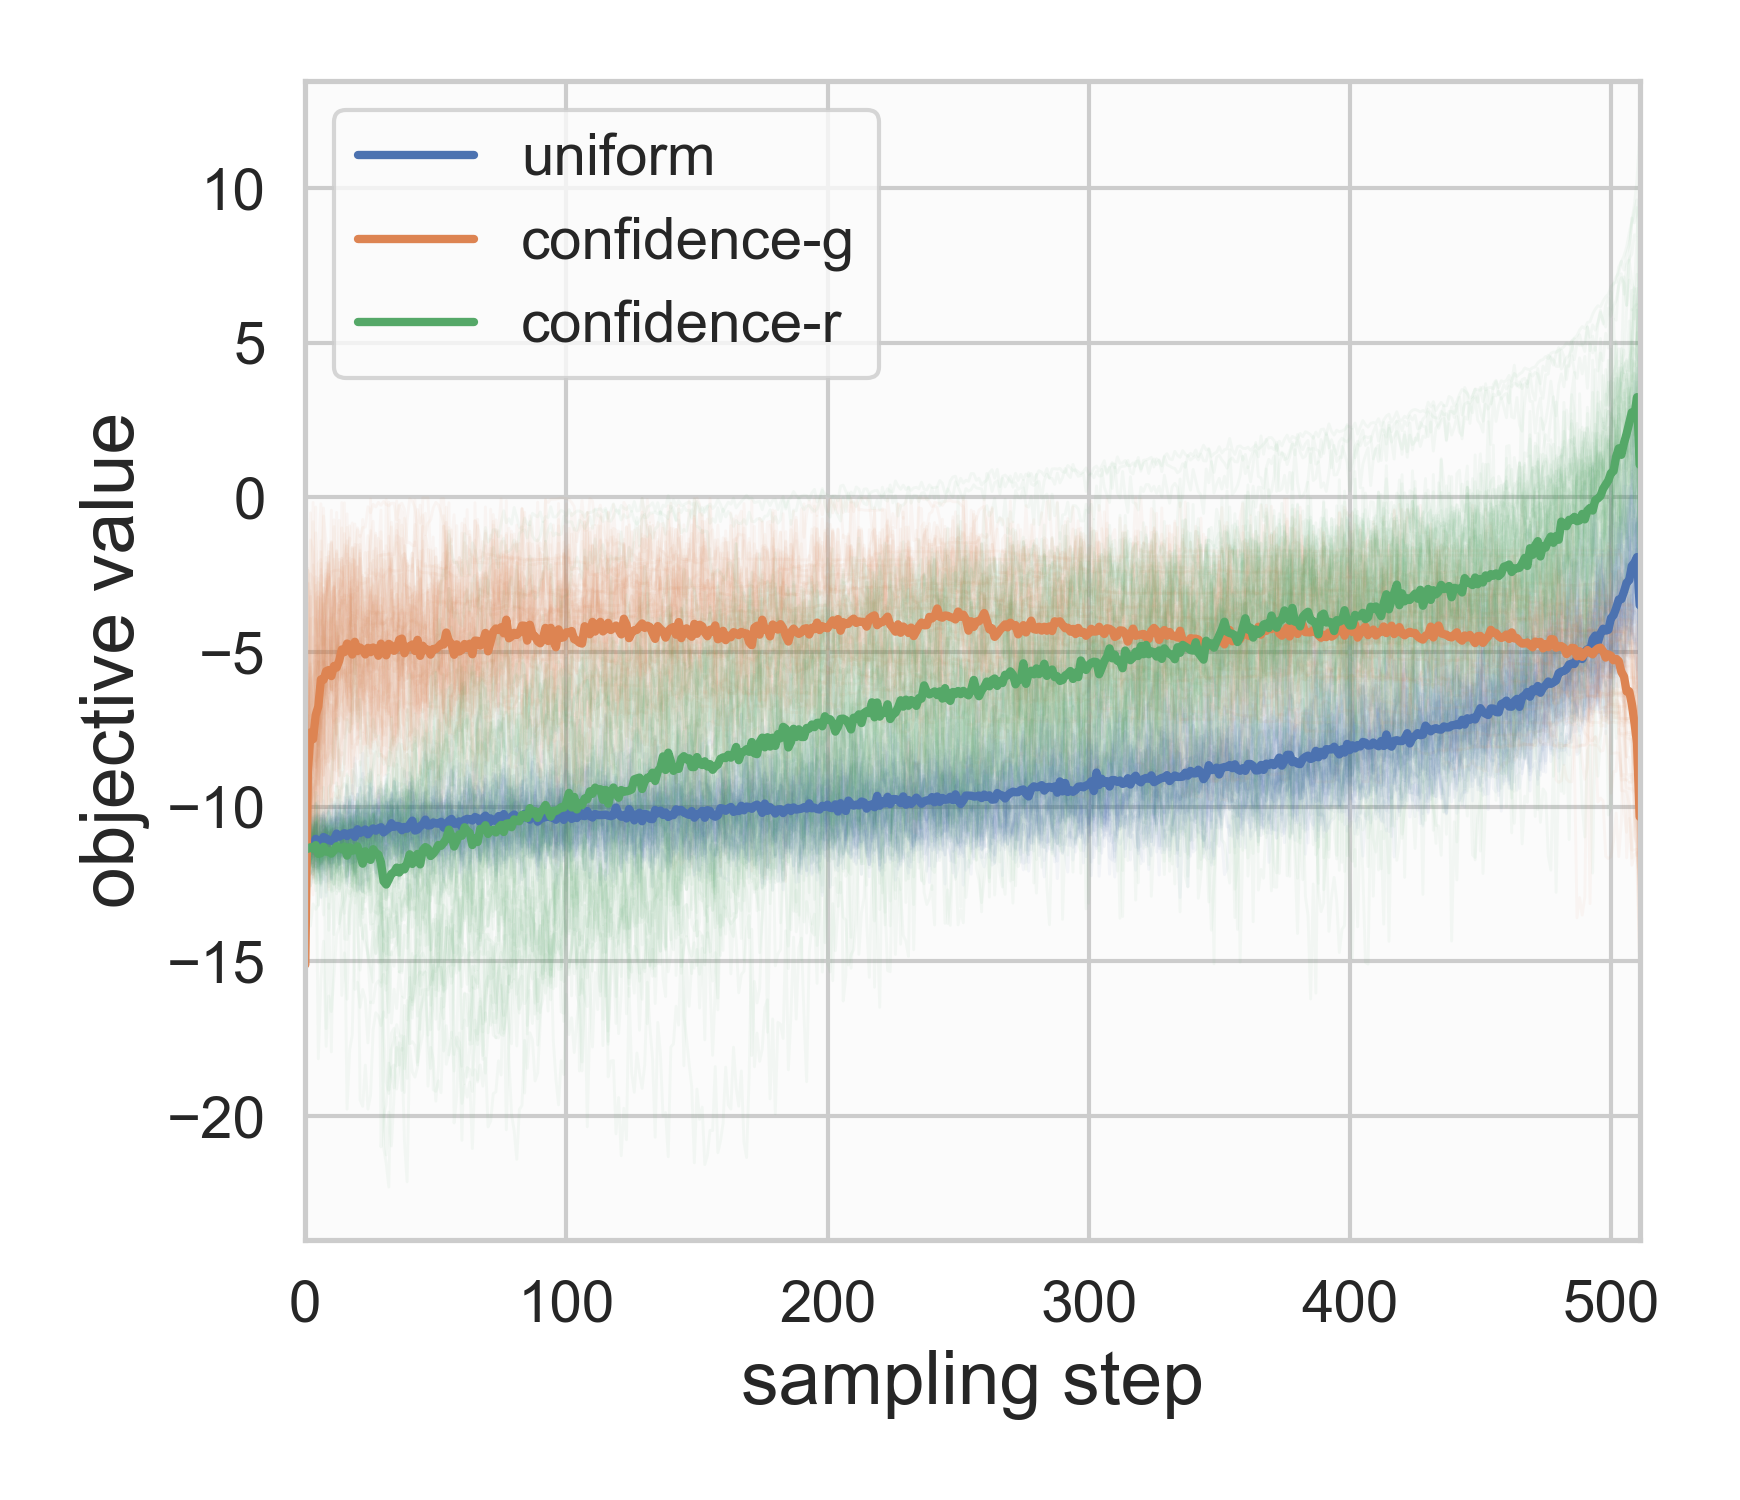
\includegraphics[width=\linewidth]{figs/objective_steps_512.png}
        \caption{512 steps}
    \end{subfigure}
    \hfill
    \begin{subfigure}[h]{0.48\linewidth}
        \centering
        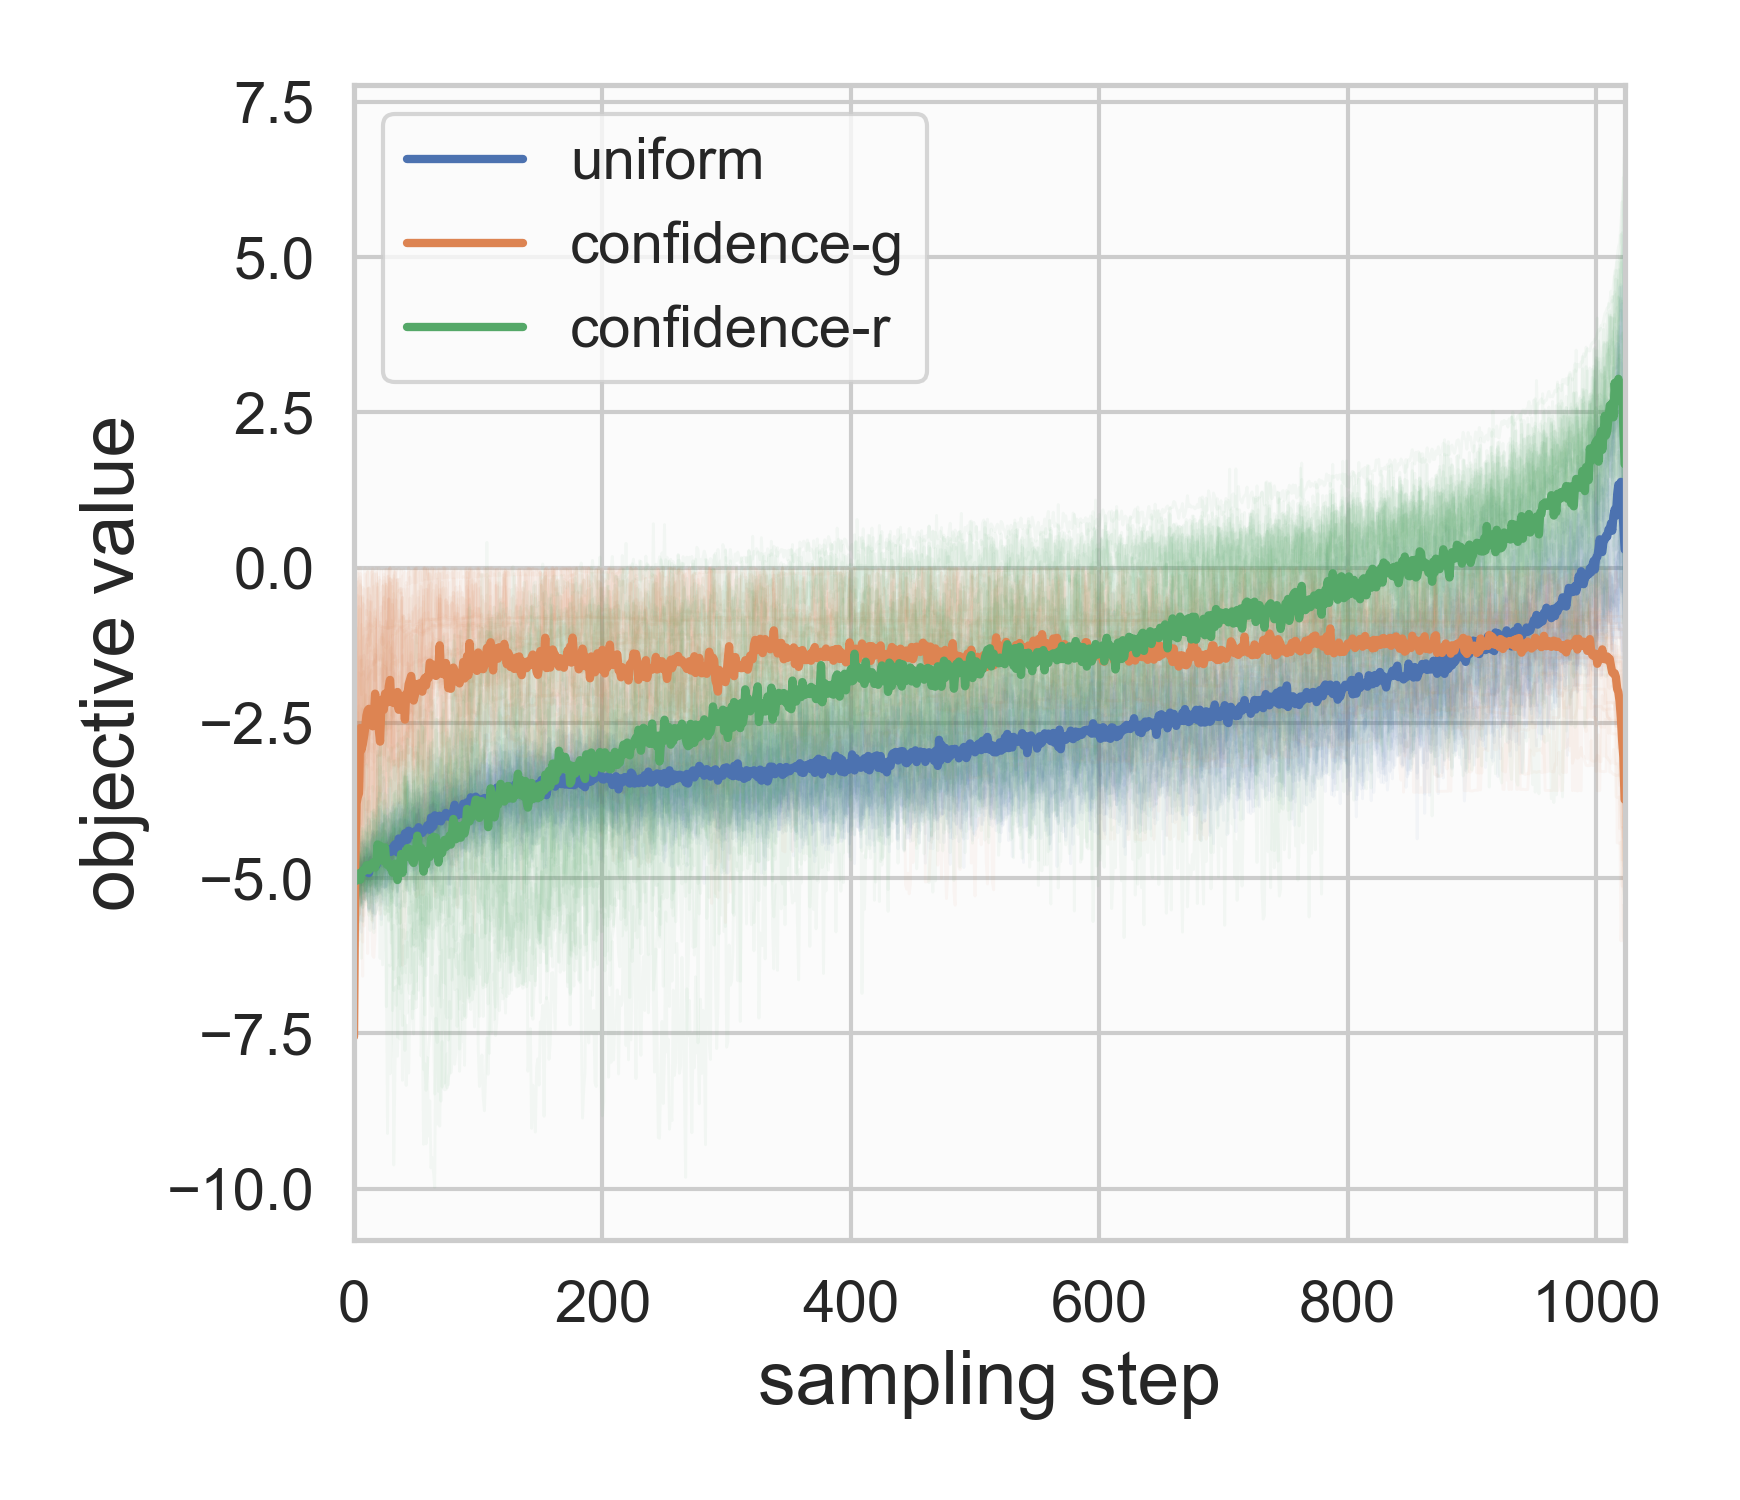
\includegraphics[width=\linewidth]{figs/objective_steps_1024.png}
        \caption{1024 steps}
    \end{subfigure}
    \caption{Local objective values \eqref{eq:trainable_confidence} attained by different unmasking methods in text generation with RADD~\citep{ou2025absorbingdiscretediffusionsecretly}.}
    \label{fig:radd-obj-all-step}
\end{figure}

\subsection{Evaluation of VLP}\label{sec:vlp}

\subsubsection{Experiment Setup}\label{sec:vlp-experiment-setup}

\paragraph{Text Generation Details.}

For the RADD text generation experiments, we use the pretrained checkpoint corresponding to the small RADD configuration with 12 Transformer blocks, hidden size 768, 12 attention heads, sequence length 1024, and approximately 162M parameters. The backbone is kept frozen throughout policy training. The policy network follows Section~\ref{subsec:architecture}, with approximately 5.3M trainable parameters, about 3\% of the RADD backbone.

We train the policy on OpenWebText. Text is tokenized with the GPT-2 tokenizer, appended with EOS tokens, concatenated, and split into fixed-length chunks of 1024 tokens. Since this is unconditional generation, there is no prompt portion and all positions are eligible for masking or unmasking. Unless otherwise specified, policy training uses batch size 4, one gradient accumulation step, and \(K=32\) discrete masking steps for the RADD runs used in our reported sampling experiments. We optimize with AdamW using learning rate \(3\times 10^{-4}\), weight decay 0, \((\beta_1,\beta_2)=(0.9,0.999)\), \(\epsilon=10^{-8}\), gradient clipping at norm 1.0, and EMA decay 0.9999 for the policy parameters. The KL regularization parameter $\lambda$ is set to $10^{-2}$. Training is run on a single A100 80GB GPU for $2\times10^3$ steps.

For evaluation, we generate unconditional sequences of length 1024 using the RADD diffusion sampler. We evaluate sampling budgets from 16 to 256 steps. For each setting, we generate 100 independent samples and report the mean and standard deviation of GPT-2-large perplexity. We compare uniform unmasking, greedy margin-based confidence unmasking, randomized margin-based confidence unmasking, and the learned policy.


\paragraph{Code and Math Generation Details.}

For both 7B models, we evaluate HumanEval~\citep{chen2021evaluatinglargelanguagemodels}, MBPP~\citep{austin2021programsynthesislargelanguage}, GSM8K~\citep{cobbe2021training}, and MATH500~\citep{lightman2023let}. HumanEval and MBPP are evaluated using Pass@1 ($\uparrow$), while GSM8K and MATH500 are evaluated using final-answer accuracy ($\uparrow$). All evaluations are run through the LM Evaluation Harness with our DiffuCoder wrapper.

The policy is trained on instruction-output pairs from OpenCoder-SFT~\citep{Gokaslan2019OpenWeb} and MetaMathQA~\citep{yu2023metamath}. Each example is converted to the chat format shown in Table~\ref{tab:chat-sft}. We tokenize each formatted sequence with the corresponding model tokenizer, truncate or pad to length 1024, and construct a prompt mask marking all tokens before the assistant response. During training and inference, prompt tokens are kept fixed; only response tokens are masked, unmasked, or generated.

The backbone model is loaded in \texttt{bfloat16} and kept frozen throughout policy training. The trained policy is a lightweight transformer policy network as described in Section~\ref{subsec:architecture}, with approximately 115.7M parameters or about 1.5\% of the 7.6B-parameter backbone.

Unless otherwise specified, we train the policy with batch size 4, sequence length 1024, and \(K=16\) discrete masking steps. We optimize the policy with AdamW using learning rate \(10^{-3}\), weight decay 0, \((\beta_1,\beta_2)=(0.9,0.999)\), \(\epsilon=10^{-8}\), and gradient clipping at norm $1.0$. The KL regularization parameter $\lambda$ is set to $10^{-2}$. Training is run on a single A100 80GB GPU for $10^3$ steps.

For evaluation, prompts are formatted with the chat template (Table~\ref{tab:chat-humaneval}, \ref{tab:chat-mbpp}) and padded with mask tokens up to the requested generation length. We use context length 1024 for code tasks (HumanEval, MBPP) and 512 for math tasks (GSM8K, MATH500). Generation uses the diffusion sampler for the specified number of steps. For confidence and policy variants, an algorithm temperature controls whether positions are selected greedily or sampled from a softmax over scores. Unless otherwise specified, the temperature for performing categorical sampling among the vocabulary is set to $0$.


\subsubsection{Additional Results}\label{sec:vlp-additional-results}

\paragraph{Evaluation on DiffuCoder-7B.} Table~\ref{tab:diffucoder-all} reports the corresponding full DiffuCoder-7B results on HumanEval, MBPP, GSM8K, and MATH500. This table expands the main-text summary by including all step counts and both confidence variants. VLP consistently improves over uniform unmasking and is especially strong on HumanEval and MATH500, while randomized confidence remains a competitive baseline on some MBPP and GSM8K settings.

\paragraph{Effect of KL regularization in VLP training.} Table~\ref{tab:text-kl} studies the effect of the KL regularization strength $\lambda$ in RADD text generation with diffusion steps $K$ for training fixed at 16. We evaluate unconditional generation quality using perplexity and entropy across different sampling steps. The best value of $\lambda$ depends on the inference budget: $\lambda=10^{-2}$ gives the lowest perplexity at 16 steps, while $\lambda=10^{-1}$ gives the lowest perplexity at 32, 64, and 128 steps. This suggests that KL regularization consistently brings improvement to generation quality.

\paragraph{Effect of sampling steps $K$ in VLP training.} Table~\ref{tab:text-step} ablates the choice of the training diffusion step $K$ for RADD, with $\lambda$ fixed at $1e^{-2}$. Although each policy is trained with a fixed $K$, we evaluate it across several sampling budgets. Training with $K=32$ gives the strongest overall perplexity, suggesting that a mid-range training horizon transfers well across different numbers of inference steps.

\paragraph{Effect of sampling temperature.} The generation process involves two types of temperature: (1) vocabulary temperature that controls the categorical sampling among the vocabulary, and (2) policy temperature that controls the greediness of choosing unmasking indices from the predicted multinomial distribution. Table~\ref{tab:temp-humaneval} studies the effect of varying both types of temperatures on Pass@1 score of HumanEval with DiffuCoder-7B model. The results show that low vocabulary temperature is important for reliable code generation, while a moderate policy temperature can improve Pass@1 by avoiding overly deterministic position selection.


\begin{table*}[h]
\centering
\caption{Results ($\uparrow$) of DiffuCoder-7B under different unmasking strategies and numbers of sampling steps across four benchmarks.}
\setlength{\tabcolsep}{4.5pt}
\resizebox{\textwidth}{!}{%
\begin{tabular}{ccccccccccccccccc}
\toprule
& \multicolumn{4}{c}{HumanEval}
& \multicolumn{4}{c}{MBPP}
& \multicolumn{4}{c}{GSM8K}
& \multicolumn{4}{c}{MATH500} \\
\cmidrule(lr){2-5}\cmidrule(lr){6-9}\cmidrule(lr){10-13}\cmidrule(lr){14-17}
steps
& 16 & 32 & 64 & 128
& 16 & 32 & 64 & 128
& 16 & 32 & 64 & 128
& 16 & 32 & 64 & 128 \\
\midrule
uniform
& 15.9 & 23.8 & 22.6 & 28.7
& 23.8 & 31.6 & 35.8 & 39.4
& 7.1 & 7.3 & 8.8 & 9.1
& 3.8 & 4.6 & 5.4 & 6.4 \\
confidence-g
& 4.3 & 11.6 & 26.2 & 30.2
& 1.8 & 5.0 & 18.4 & 31.2
& 2.4 & 3.8 & 6.4 & 6.4
& 1.4 & 1.4 & 2.4 & 3.0 \\
confidence-r
& 20.7 & 25.0 & 29.9 & 32.3
& \textbf{33.2} & \textbf{39.4} & 39.8 & 41.8
& 7.3 & \textbf{10.2} & \textbf{10.5} & \textbf{10.4}
& 4.2 & 5.8 & 5.0 & 6.0 \\
\midrule
\cellcolor{lightblue}VLP
& \cellcolor{bestgreen}\textbf{23.2} & \cellcolor{bestgreen}\textbf{27.4} & \cellcolor{bestgreen}\textbf{30.5} & \cellcolor{bestgreen}\textbf{33.5}
& \cellcolor{lightblue}29.8 & \cellcolor{lightblue}37.6 & \cellcolor{bestgreen}\textbf{40.4} & \cellcolor{bestgreen}\textbf{42.4}
& \cellcolor{bestgreen}\textbf{7.4} & \cellcolor{lightblue}9.7 & \cellcolor{lightblue}10.2 & \cellcolor{bestgreen}\textbf{10.4}
& \cellcolor{bestgreen}\textbf{6.4} & \cellcolor{bestgreen}\textbf{8.8} & \cellcolor{bestgreen}\textbf{8.2} & \cellcolor{bestgreen}\textbf{7.0} \\
\bottomrule
\end{tabular}%
}
\label{tab:diffucoder-all}
\end{table*}


\begin{table*}[h]
\centering
\caption{Effect of KL regularization strength $\lambda$ in VLP training for RADD. We report perplexity ($\downarrow$) and entropy of unconditional generation at different sampling steps.}
\setlength{\tabcolsep}{4.5pt}
\begin{tabular}{ccccccccc}
\toprule
& \multicolumn{4}{c}{Perplexity}
& \multicolumn{4}{c}{Entropy} \\
\cmidrule(lr){2-5}\cmidrule(lr){6-9}
$\lambda$
& 16 & 32 & 64 & 128
& 16 & 32 & 64 & 128 \\
\midrule
0
& 313.9 & 186.0 & 142.5 & 127.4
& 5.79 & 5.73 & 5.68 & 5.68 \\
$10^{-3}$
& 320.0 & 182.8 & 140.5 & 129.8
& 5.78 & 5.73 & 5.68 & 5.66 \\
$10^{-2}$
& \textbf{301.7} & 186.8 & 145.3 & 127.3
& 5.77 & 5.73 & 5.68 & 5.67 \\
$10^{-1}$
& 301.8 & \textbf{179.1} & \textbf{134.4} & \textbf{118.6}
& 5.77 & 5.72 & 5.67 & 5.64 \\
\bottomrule
\end{tabular}
\label{tab:text-kl}
\end{table*}

\begin{table*}[h]
\centering
\caption{Effect of choice of $K$ in VLP training for RADD. We report perplexity ($\downarrow$) and entropy of unconditional generation at different sampling steps.}
\setlength{\tabcolsep}{4.5pt}
\begin{tabular}{ccccccccc}
\toprule
& \multicolumn{4}{c}{Perplexity}
& \multicolumn{4}{c}{Entropy} \\
\cmidrule(lr){2-5}\cmidrule(lr){6-9}
$K$
& 16 & 32 & 64 & 128
& 16 & 32 & 64 & 128 \\
\midrule
16
& 302.5 & 184.6 & 146.8 & \textbf{125.4}
& 5.76 & 5.73 & 5.69 & 5.67 \\
32
& \textbf{300.8} & \textbf{174.8} & \textbf{138.0} & 128.9
& 5.78 & 5.72 & 5.67 & 5.67 \\
64
& 316.2 & 178.1 & 141.8 & 125.5
& 5.78 & 5.72 & 5.69 & 5.66 \\
\bottomrule
\end{tabular}
\label{tab:text-step}
\end{table*}


\iffalse
\begin{table*}[h]
\caption{Average perplexity ($\downarrow$) of unconditional generations from RADD under different unmasking strategies and numbers of sampling steps. All generations have context length 1024.}
\centering
\begin{tabular}{cccccc}
\toprule
steps & 16 & 32 & 64 & 128 & 256 \\
\midrule
uniform
& 335.1\scriptsize{$\pm$85.3}
& 199.7\scriptsize{$\pm$50.8}
& 154.5\scriptsize{$\pm$52.8}
& 132.2\scriptsize{$\pm$42.9}
& 118.9\scriptsize{$\pm$38.4} \\
confidence-g
& 836.3\scriptsize{$\pm$226.7}
& 800.0\scriptsize{$\pm$283.9}
& 618.5\scriptsize{$\pm$213.0}
& 782.0\scriptsize{$\pm$316.4}
& 644.3\scriptsize{$\pm$312.1} \\
confidence-r
& 308.7\scriptsize{$\pm$96.6}
& 186.3\scriptsize{$\pm$57.7}
& 132.4\scriptsize{$\pm$39.0}
& \textbf{109.2}\scriptsize{$\pm$29.6}
& \textbf{103.4}\scriptsize{$\pm$36.9} \\
\midrule
\alg{}
& \textbf{293.2}\scriptsize{$\pm$71.7}
& \textbf{179.6}\scriptsize{$\pm$47.3}
& \textbf{130.3}\scriptsize{$\pm$33.4}
& 116.9\scriptsize{$\pm$34.2}
& 106.7\scriptsize{$\pm$36.8} \\
\bottomrule
\end{tabular}
\label{tab:text-gen}
\end{table*}

\begin{table*}[h!]
\centering
\caption{Pass@1 ($\uparrow$) of DiffuCoder-7B under different unmasking strategies and numbers of sampling steps on coding benchmarks. All generations have context length 1024.}
\begin{tabular}{ccccccccc}
\toprule
& \multicolumn{4}{c}{HumanEval} & \multicolumn{4}{c}{MBPP} \\
\cmidrule(lr){2-5}\cmidrule(lr){6-9}
steps
& 16 & 32 & 64 & 128
& 16 & 32 & 64 & 128 \\
\midrule
uniform
& 15.9 & 23.8 & 22.6 & 28.7
& 23.8 & 31.6 & 35.8 & 39.4 \\
confidence-g
& 4.3 & 11.6 & 26.2 & 30.2
& 1.8 & 5.0 & 18.4 & 31.2 \\
confidence-r
& 20.7 & 25.0 & 29.9 & 32.3
& \textbf{33.2} & \textbf{39.4} & 39.8 & 41.8 \\
\midrule
VLP
& \textbf{23.2} & \textbf{27.4} & \textbf{30.5} & \textbf{33.5}
& 29.8 & 37.6 & \textbf{40.4} & \textbf{42.4} \\
\bottomrule
\end{tabular}
\label{tab:code-gen-diffucoder}
\end{table*}

\begin{table*}[h!]
\centering
\caption{Zero-shot math results ($\uparrow$) of DiffuCoder under different unmasking strategies and numbers of sampling steps.}
\begin{tabular}{ccccccccc}
\toprule
& \multicolumn{4}{c}{GSM8K} & \multicolumn{4}{c}{MATH500} \\
\cmidrule(lr){2-5}\cmidrule(lr){6-9}
steps
& 16 & 32 & 64 & 128
& 16 & 32 & 64 & 128 \\
\midrule
confidence-r
& 7.3 & 10.2 & -- & --
& 4.2 & 5.8 & 5.0 & 6.0 \\
uniform
& 7.1 & 7.3 & -- & --
& 3.8 & 4.6 & 5.4 & 6.4 \\
VLP
& \textbf{7.4} & 9.7 & -- & --
& \textbf{6.4} & \textbf{8.8} & \textbf{8.2} & \textbf{7.0} \\
\bottomrule
\end{tabular}
\label{tab:math-diffucoder}
\end{table*}

\begin{table*}[h]
\centering
\caption{Pass@1 ($\uparrow$) of Dream~7B under different unmasking strategies and numbers of sampling steps on coding benchmarks. Here ``origin'' denotes Dream's original sampling strategy and ``dream-policy'' denotes our trained policy.}
\begin{tabular}{ccccccccc}
\toprule
& \multicolumn{4}{c}{HumanEval} & \multicolumn{4}{c}{MBPP} \\
\cmidrule(lr){2-5}\cmidrule(lr){6-9}
steps
& 16 & 32 & 64 & 128
& 16 & 32 & 64 & 128 \\
\midrule
confidence
& 15.2 & 18.3 & 26.2 & 27.4
& 25.2 & 24.4 & 27.4 & 32.0 \\
origin
& 8.5 & 17.6 & 19.5 & 23.2
& 18.6 & 25.6 & 27.6 & 30.8 \\
VLP
& \textbf{17.0} & \textbf{22.6} & \textbf{27.4} & \textbf{29.3}
& 22.8 & \textbf{26.2} & \textbf{31.6} & \textbf{32.8} \\
\bottomrule
\end{tabular}
\label{tab:dream-code}
\end{table*}

\begin{table*}[h]
\centering
\caption{Math benchmark results ($\uparrow$) of Dream~7B under different unmasking strategies and numbers of sampling steps.}
\begin{tabular}{ccccccccc}
\toprule
& \multicolumn{4}{c}{GSM8K} & \multicolumn{4}{c}{MATH500} \\
\cmidrule(lr){2-5}\cmidrule(lr){6-9}
steps
& 16 & 32 & 64 & 128
& 16 & 32 & 64 & 128 \\
\midrule
confidence-r
& 32.7 & 36.5 & \textbf{39.2} & \textbf{39.6}
& 15.2 & 16.8 & 16.6 & 18.2 \\
uniform
& 23.4 & 30.0 & 34.9 & 35.4
& 10.4 & 12.8 & 13.8 & 16.8 \\
VLP
& \textbf{33.6} & \textbf{36.6} & 38.3 & 38.2
& \textbf{15.6} & \textbf{17.0} & \textbf{17.2} & \textbf{19.4} \\
\bottomrule
\end{tabular}
\label{tab:dream-math}
\end{table*}
\fi


\subsubsection{Chat Template for Code Generation Experiments}
\begin{table*}[h]
\centering
\begin{minipage}[t]{0.48\textwidth}
\centering
\caption{Temperature analysis on HumanEval. We report Pass@1 ($\uparrow$) at different sampling steps.}
\setlength{\tabcolsep}{4.5pt}
\begin{tabular}{cccc}
\toprule
& & \multicolumn{2}{c}{Steps} \\
\cmidrule(lr){3-4}
Temperature type & Value & 16 & 32 \\
\midrule
\multirow{6}{*}{Vocabulary}
& 0.0 & \textbf{23.2} & 25.0 \\
& 0.1 & 18.9 & \textbf{32.3} \\
& 0.2 & 19.5 & 28.0 \\
& 0.5 & 15.2 & 22.6 \\
& 0.8 & 11.0 & 22.6 \\
& 1.0 & 7.9 & 11.6 \\
\midrule
\multirow{10}{*}{Policy}
& 0.1 & 13.4 & 24.4 \\
& 0.2 & 18.9 & 25.0 \\
& 0.3 & 20.7 & 26.8 \\
& 0.4 & \textbf{25.0} & \textbf{27.4} \\
& 0.5 & 23.2 & \textbf{27.4} \\
& 0.6 & 22.6 & 23.2 \\
& 0.7 & 21.3 & 22.0 \\
& 0.8 & 20.7 & 25.0 \\
& 0.9 & 18.3 & 23.2 \\
& 1.0 & 17.1 & 24.4 \\
\bottomrule
\end{tabular}
\label{tab:temp-humaneval}
\end{minipage}
\hfill
\begin{minipage}[t]{0.48\textwidth}
\centering
\caption{Chat template for \alg{} OpenCoder-SFT training.}
\begin{chatbox}
    <|im\_start|>system\\
    You are a helpful assistant.<|im\_end|>\\
    <|im\_start|>user\\
    \{{query}\}\\
    <|im\_end|>\\
    <|im\_start|>assistant\\
    \{output\}\\
    <|im\_end|>
\end{chatbox}
\label{tab:chat-sft}
\end{minipage}

\vspace{0.8em}

\begin{minipage}[t]{0.48\textwidth}
\centering
\caption{Chat template for \alg{} HumanEval evaluation.}
\begin{chatbox}
    <|im\_start|>system\\
    You are a helpful assistant.<|im\_end|>\\
    <|im\_start|>user\\
    Please complete the following problem:\\
    \textasciigrave\textasciigrave\textasciigrave\\
    \{prompt\}\\
    \textasciigrave\textasciigrave\textasciigrave\\
    <|im\_end|>\\
    <|im\_start|>assistant\\
    Here is the code to solve this problem:\\
    \textasciigrave\textasciigrave\textasciigrave python
\end{chatbox}
\label{tab:chat-humaneval}
\end{minipage}
\hfill
\begin{minipage}[t]{0.48\textwidth}
\centering
\caption{Chat template for \alg{} MBPP evaluation.}
\begin{chatbox}
    <|im\_start|>system\\
    You are a helpful assistant.<|im\_end|>\\
    <|im\_start|>user\\
    \textasciigrave\textasciigrave\textasciigrave\\
    \{{prompt}\}\\
    \textasciigrave\textasciigrave\textasciigrave\\
    <|im\_end|>\\
    <|im\_start|>assistant\\
    Here is the code to solve this problem:\\
    \textasciigrave\textasciigrave\textasciigrave python
\end{chatbox}
\label{tab:chat-mbpp}
\end{minipage}
\end{table*}
